\documentclass[xcolor=x11names,handout]{beamer}
\includeonlyframes{current}
\usepackage{hyperref}
\hypersetup{
    colorlinks=true,
    linkcolor=blue,
    filecolor=magenta,      
    urlcolor=cyan,
}
\usepackage{mybeamer}
\usepackage{mystyle}
\usepackage{bm}
\usepackage{tikz}
\usepackage{adjustbox}
\usepackage{booktabs}       % professional-quality tables
\usepackage{circuitikz}
\setbeamercovered{transparent}
\usetikzlibrary{calc,shapes,positioning}
\usetikzlibrary{arrows}
\usetikzlibrary{fit}
\newcommand{\midarrow}{\tikz \draw[-triangle 90] (0,0) -- +(.1,0);}
% set arrow type and size by tikz
% alternative to 'Straight Barb' can be 'Latex, Stealth, Computer Modern Rightarrow'.
\usetikzlibrary{arrows.meta}
\tikzset{>={Straight Barb[width=1.3mm,length=1.3mm]}}
\tikzset{block/.style = {draw, fill=white, rectangle,
                  minimum height=3em, minimum width=2cm},
        input/.style = {coordinate},
        output/.style = {coordinate},
        pinstyle/.style = {pin edge={to-,t,black}}
    }

\newcommand{\ubar}[1]{\mkern2mu\underline{\mkern-2mu #1\mkern-2mu}\mkern2mu}
\begin{document}


\begin{frame}
  \title{Perspectives on Probabilistic Graphical Models}
  \subtitle{}
  % \includegraphics[height=1cm,width=2cm]{kth_eng_cmyk_wireless.eps}
  \author{ \small Dong Liu
    \\
    \vspace{0.3cm}
    {\it \scriptsize Information Science and Engineering \\
      KTH - Royal Institute of Technology}
    \vspace{0.3cm}
  }
  \vspace{-0.5cm}
  \date{
    \includegraphics[height=2cm,angle=0]{kth_eng_cmyk_wireless.eps}  \\
    % \vspace{0.3cm}
    \scriptsize
    \begin{itemize}
    \item Profile page: \href{https://firsthandscientist.github.io/}{https://firsthandscientist.github.io/} \\
    \item Slide is available at: \href{https://github.com/FirstHandScientist/phdthesis}{https://github.com/FirstHandScientist/phdthesis}
    \end{itemize} }
  \titlepage
  
\end{frame}

% decrease the size of font
\scriptsize
%%%%%%%%%%%%%%%%%%%%%%%%%%%%%%%%%%%%%%%%%%%%%%%%%%%%%% 
% ------------------------------------------------
%   Seciton motivation
%%%%%%%%%%%%%%%%%%%%%%%%%%%%%%%%%%%%%%%%%%%%%%%%%%%%%% 


\section{Motivation}

{ \setbeamercolor{background canvas}{bg=hl_bg}
  \setbeamercolor{normal text}{fg=hl_fg}
  \setbeamercolor{frametitle}{fg=hl_fg}
  \begin{frame}
    \usebeamercolor[fg]{normal text}
    \begin{center}
      {\large Why are Probabilistic Graphical Models interested?}
    \end{center}
  \end{frame}
}
\subsection{Directed}
\begin{frame}[label=current]{Directed Graph Representation}
  \begin{itemize}
    
    \item 
      \begin{columns}
        \column{0.5\textwidth}
        \hskip 1cm
        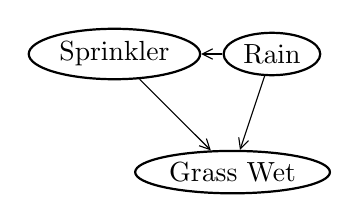
\begin{tikzpicture}
          % \tikzstyle{enode} = [thick, draw=blue, circle, inner sep = 3pt,
          % align=center]
          \tikzstyle{enode} = [thick, draw=black, ellipse, inner sep = 2pt,  align=center]
          \tikzstyle{nnode} = [thick, rectangle, rounded corners = 2pt, minimum size = 0.5cm,draw,inner sep = 2pt]

          \node[enode] (s) at (-0.5, 1.5) {Sprinkler};
          \node[enode] (r) at (1.5, 1.5) {Rain};
          \node[enode] (gw) at (1, 0) {Grass Wet};
          \draw[->] (r) to (s);
          \draw[->] (r) to (gw);
          \draw[->] (s) to (gw);
        \end{tikzpicture}\\
        \centering
        Is the sprinkler working?
        
        \column{0.5\textwidth}
        \hskip -1cm
        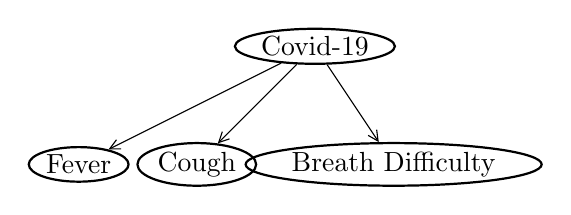
\begin{tikzpicture}
          \tikzstyle{cnode} = [thick, draw=black, ellipse, inner sep = 1pt,  align=center]
          \tikzstyle{nnode} = [thick, rectangle, rounded corners = 0pt,draw,inner sep = 2pt]
          \node[cnode] (virus) at (0, 1.5) {Covid-19};
          \node[cnode] (fever) at (-3, 0) {Fever};
          \node[cnode] (cough) at (-1.5, 0) {Cough};
          \node[cnode] (breath) at (1, 0) {Breath Difficulty};
          \draw[->] (virus) -- (fever);
          \draw[->] (virus) -- (cough);
          \draw[->] (virus) -- (breath);
        \end{tikzpicture}\\
        \centering
        Is the person get contiguous by COVID?
      \end{columns}
    \item 
      \vskip 0.5cm
      \begin{columns}
        \column{0.5\textwidth}
        \hskip 1cm
        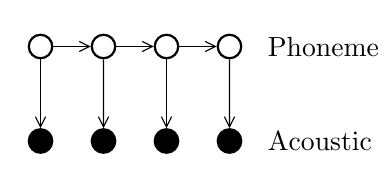
\begin{tikzpicture}[scale=0.8]
          \tikzstyle{enode} = [thick, draw, circle, inner sep = 3pt,  align=center]
          \tikzstyle{cnode} = [thick, fill=black, draw, circle, inner sep = 3pt,  align=center]
          \begin{scope}{scale=0.5, xshift=1cm}
            \node[enode] (x1) at (-2, 0) {};
            \node[enode] (x2) at (-1, 0) {};
            \node[enode] (x3) at (0, 0) {};
            \node[enode] (x4) at (1, 0) {};
            \node[text width=1cm, right = 0.2cm of x4] {Phoneme};
            \node[cnode] (y1) at (-2, -1.5) {};
            \node[cnode] (y2) at (-1, -1.5) {};
            \node[cnode] (y3) at (0, -1.5) {};
            \node[cnode] (y4) at (1, -1.5) {};
            \node[text width=1cm, right = 0.2cm of y4] {Acoustic};

            \draw[->] (x1) to (x2);
            \draw[->] (x2) to (x3);
            \draw[->] (x3) to (x4);

            \draw[->] (x1) to (y1);
            \draw[->] (x2) to (y2);
            \draw[->] (x3) to (y3);
            \draw[->] (x4) to (y4);

          \end{scope}
        \end{tikzpicture}
        \vskip 0.1cm
        \centering
        Speech Recognition
        \column{0.5\textwidth}
        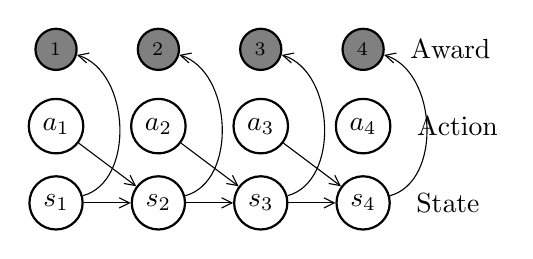
\begin{tikzpicture}[scale=0.65]
          \tikzstyle{enode} = [thick, draw, circle, inner sep = 3pt,  align=center]
          \tikzstyle{cnode} = [thick, fill=gray, draw, circle, inner sep = 3pt,  align=center]
          \begin{scope}{scale=0.5, xshift=1cm}
            \node[cnode] (o1) at (-2, 1.5) {$\Oo_1$};
            \node[cnode] (o2) at (0, 1.5) {$\Oo_2$};
            \node[cnode] (o3) at (2, 1.5) {$\Oo_3$};
            \node[cnode] (o4) at (4, 1.5) {$\Oo_4$};
            \node[text width=1cm, right = 0.2cm of o4] {Award};

            \node[enode] (a1) at (-2, 0) {$a_1$};
            \node[enode] (a2) at (0, 0) {$a_2$};
            \node[enode] (a3) at (2, 0) {$a_3$};
            \node[enode] (a4) at (4, 0) {$a_4$};
            \node[text width=1cm, right = 0.2cm of a4] {Action};
            \node[enode] (s1) at (-2, -1.5) {$s_1$};
            \node[enode] (s2) at (0, -1.5) {$s_2$};
            \node[enode] (s3) at (2, -1.5) {$s_3$};
            \node[enode] (s4) at (4, -1.5) {$s_4$};
            \node[text width=1cm, right = 0.2cm of s4] {State};

            \draw[->] (s1) to (s2);
            \draw[->] (s2) to (s3);
            \draw[->] (s3) to (s4);
            \draw[->] (a1) to (s2);
            \draw[->] (a2) to (s3);
            \draw[->] (a3) to (s4);
            \draw[->] (s1) to [out=15, in=-15] (o1);
            \draw[->] (s2) to [out=15, in=-15] (o2);
            \draw[->] (s3) to [out=15, in=-15] (o3);
            \draw[->] (s4) to [out=15, in=-15] (o4);

          \end{scope}
          
        \end{tikzpicture}
        \centering
        Control, reinforcement learning        
      \end{columns}
    
  \end{itemize}

\end{frame}


\subsection{Directed}
\begin{frame}[label=current]{Undirected Graph Representations}
  \begin{itemize}
  \item % image segmentation
        \begin{tikzpicture}
          \tikzstyle{enode} = [thick, draw, circle, inner sep = 3pt,  align=center]
          \tikzstyle{cnode} = [thick, fill=gray, draw, circle, inner sep = 3pt,  align=center]
          \begin{scope}{scale=0.4}
            \node[inner sep=0pt] (img) at (-7,0) {\includegraphics[width=.25\textwidth]{images/illustrate/slam_img.png}};
          \end{scope}
          \begin{scope}{scale=0.4}
            \node[inner sep=0pt] (slam) at (0,0) {\includegraphics[width=.25\textwidth]{images/illustrate/slam_lab.png}};
          \end{scope}
          
          \begin{scope}[local bounding box=crf, scale=0.6, xshift=-4cm]
            \node[enode] (x1) at (-2, 1) {};
            \node[enode] (x2) at (0, 1) {};
            \node[enode] (x3) at (-2, -1) {};
            \node[enode] (x4) at (0, -1) {};

            \node[cnode] (y1) at (-3, 0) {};
            \node[cnode] (y2) at (-1, 0) {};
            \node[cnode] (y3) at (-3, -2) {};
            \node[cnode] (y4) at (-1, -2) {};
            \node[text width=1cm, left = 0.2cm of x1] {Label};
            \node[text width=1cm, right = 0.2cm of y4] {Pixel};

            \draw[-] (x1) to (y1);
            \draw[-] (x2) to (y2);
            \draw[-] (x3) to (y3);
            \draw[-] (x4) to (y4);

            \draw[-] (x1) to (x2);
            \draw[-] (x1) to (x3);
            \draw[-] (x2) to (x4);
            \draw[-] (x3) to (x4);
          \end{scope}
          
        \end{tikzpicture}
        \vskip 0.1cm
        \centering
        Vision Perception
        \item % digital communication
        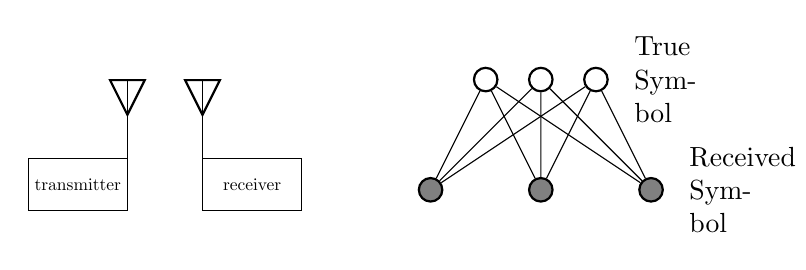
\begin{tikzpicture}[scale=0.7]
          \tikzstyle{enode} = [thick, draw, circle, inner sep = 3pt,  align=center]
          \tikzstyle{cnode} = [thick, fill=gray, draw, circle, inner sep = 3pt,  align=center]
      
          \begin{scope}[local bounding box=mrf]{scale=0.2}
            \node[enode] (x1) at (-2, 1) {};
            \node[enode] (x2) at (-1, 1) {};
            \node[enode] (x3) at (0, 1) {};

            \node[cnode] (y1) at (-3, -1) {};
            \node[cnode] (y2) at (-1, -1) {};
            \node[cnode] (y3) at (1, -1) {};
            
            \node[text width=1cm, right = 0.2cm of x3] {True Symbol};
            \node[text width=1cm, right = 0.2cm of y3] {Received Symbol};

            \draw[-] (x1) to (y1);
            \draw[-] (x1) to (y2);
            \draw[-] (x1) to (y3);

            \draw[-] (x2) to (y1);
            \draw[-] (x2) to (y2);
            \draw[-] (x2) to (y3);

            \draw[-] (x3) to (y1);
            \draw[-] (x3) to (y2);
            \draw[-] (x3) to (y3);

          \end{scope}

          \begin{scope}[shift={(-4,0)}, scale=0.9, every node/.append style={transform shape}]
          \node[block](tx) at (-6,-1) {transmitter};
          \node[antenna] at (tx.east) {};
          \node[block,right = 1.5cm of tx](rx){receiver};
          \node[antenna,xscale=-1] at (rx.west) {};
          \end{scope}
        \end{tikzpicture}
        \centering
        Digital communication
      \item % Solid physics
        \begin{columns}
          \column{0.5\textwidth}
          \centering
        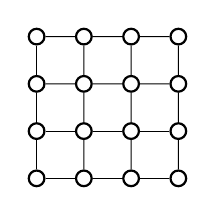
\begin{tikzpicture}
          \tikzstyle{enode} = [thick, draw, circle, inner sep = 2pt,  align=center]
          \tikzstyle{cnode} = [thick, fill=gray, draw, circle, inner sep = 3pt,  align=center]
      
          \begin{scope}[local bounding box=mrf, scale=0.6]
            \node[enode] (x11) at (0, 0) {};
            \node[enode] (x12) at (1, 0) {};
            \node[enode] (x13) at (2, 0) {};
            \node[enode] (x14) at (3, 0) {};
            \node[enode] (x21) at (0, 1) {};
            \node[enode] (x22) at (1, 1) {};
            \node[enode] (x23) at (2, 1) {};
            \node[enode] (x24) at (3, 1) {};
            \node[enode] (x31) at (0, 2) {};
            \node[enode] (x32) at (1, 2) {};
            \node[enode] (x33) at (2, 2) {};
            \node[enode] (x34) at (3, 2) {};
            \node[enode] (x41) at (0, 3) {};
            \node[enode] (x42) at (1, 3) {};
            \node[enode] (x43) at (2, 3) {};
            \node[enode] (x44) at (3, 3) {};

            \draw (x11)--(x12)--(x13)--(x14);
            \draw (x21)--(x22)--(x23)--(x24);
            \draw (x31)--(x32)--(x33)--(x34);
            \draw (x41)--(x42)--(x43)--(x44);

            \draw (x11)--(x21)--(x31)--(x41);
            \draw (x12)--(x22)--(x32)--(x42);
            \draw (x13)--(x23)--(x33)--(x43);
            \draw (x14)--(x24)--(x34)--(x44);
          \end{scope}
        \end{tikzpicture}\\
        \centering
        Physics (Ising or Potts model)
        \column{0.5\textwidth}
        \begin{itemize}[label=$\bullet$]
        \item Error-control codes
        \item Computational biology
        \item Natural language processing
        \item etc.
        \end{itemize}
      \end{columns}
  \end{itemize}


\end{frame}


%%% Local Variables:
%%% mode: latex
%%% TeX-master: "../ppgm_slide"
%%% End:

%%%%%%%%%%%%%%%%%%%%%%%%%%%%%%%%%%%%%%%%%%%%%%%%%%%%%% 
% ------------------------------------------------

%%%%%%%%%%%%%%%%%%%%%%%%%%%%%%%%%%%%%%%%%%%%%%%%%%%%%% 
% \section{Content}
% \subsection{Content}
% \begin{frame}{\large Content}
%   \begin{itemize}[label=$\bullet$]
%   \item Background: Probabilistic graphical models (PGM)
%   \item Common usage of PGMs
%   \item High-level view of inference
%   \item Play inference with neural networks
%   \item Summary
%   \end{itemize}
  
% \end{frame}



% \begin{frame}{\large Content}
%   \begin{tikzpicture}
%     \tikzstyle{enode} = [thick, draw=black, ellipse, inner sep = 2pt,  align=center]
%     \node[enode] (fd) at (0,0) {Fundamental Problems};
%     \node[enode] (fd) at (0,-1) {General Methods};
%     \node[enode] (fd) at (0,-2) {Gibbs Simpling};
%     \node[enode] (fd) at (0,-3) {Mean Field};
%     \node[enode] (fd) at (0,-4) {Loopy Belief Propagation};
%     \node[enode] (fd) at (0,-5) {Generalized Belief Propagation};
%     \node[enode] (fd) at (0,-6) {Our approximation: RENN};
%     \node[enode] (fd) at (0,-7) {Application scenarios/examples};
%     \node[enode] (fd) at (0,-8) {Some numerical results};
%   \end{tikzpicture}

% \end{frame}

%%%%%%%%%%%%%%%%%%%%%%%%%%%%%%%%%%%%%%%%%%%%%%%%%%%%%% 
% ------------------------------------------------
% section core
%%%%%%%%%%%%%%%%%%%%%%%%%%%%%%%%%%%%%%%%%%%%%%%%%%%%%% 

\section{Preliminary}
\subsection{Basics}
{ \setbeamercolor{background canvas}{bg=hl_bg}
  \setbeamercolor{normal text}{fg=hl_fg}
  \setbeamercolor{frametitle}{fg=hl_fg}
  \begin{frame}{A Guide to This Dissertation}
    \usebeamercolor[fg]{normal text}
    \centering
    \begin{tikzpicture}
      \tikzstyle{nnode} = [rectangle, rounded corners=2pt, inner sep = 6pt,  align=center]
      \tikzstyle{rnode} = [draw=black, rectangle, rounded corners=2pt, inner sep = 6pt, align=center]

      \begin{scope}[xshift=-0.5cm]
        \node[rnode, fill=white, text=black] (PandG) at (0,0) {Probability\\ \& \\ Graph};
        \node[rnode, fill=white, text=black] (mrf) at (-2,-2) {Undirected\\
          MRFs};
        \node[rnode, fill=white, text=black] (bn) at (2,-2) {Directed\\
          BNs};
        \begin{scope}[on background layer]
          \node[rnode, inner sep = 12pt, fill=gray, opacity=0.9, fit=(PandG)(mrf)(bn)] (core) {};
          \node[nnode] at (0,-1.5) {Preliminary \\ Chpt. 1, 2};
        \end{scope}
      \end{scope}
      \draw[black,->] (PandG) to (mrf);
      \draw[black,->] (PandG) to (bn);
      
      \node[rnode, fill=white, text=black] (exact) at (0, -4) {Exact Inference \\ (Briefed Chpt. 2)};
      \draw[black,->] (core) to (exact);
      
      \node[rnode, fill=white, text=black] (apprx) at (-4, -4) {Approximate Inference\\
        Chpt. 3, 4};
      \node[rnode, fill=white, text=black] (mrfLearn) at (-5, -2) {Learning\\ Chpt. 5};
      
      \draw[black,->] (mrf) to (apprx);
      \draw[black,->] (mrf) to (mrfLearn);

      \node[rnode, fill=white, text=black] (em) at (4, -4) {Learning \\ (incomplete observation) \\ Chpt. 6};
      \node[rnode, fill=white, text=black] (hmm) at (5, -2) {Temporary\\Model \\ Chpt. 7};
      \node[rnode, fill=white, text=black] (llkFree) at (4.5, 0) {Likelihood-free\\
        (Implicit) \\ Chpt. 8};
      
      \draw[black,->] (bn) to (em);
      \draw[black,->] (bn) to (hmm);
      \draw[black,->] (bn) to (llkFree);
      

      

    \end{tikzpicture}
  \end{frame}
}

\begin{frame}{What are Probabilistic Graphical Models}
  \onslide<1->{
    Informally...
    \begin{itemize}[label={$\bullet$}]
    \item attributes of our interests in a system $\rightarrow$ variable nodes
    \item relationship of these factors $\rightarrow$ structures of a graph
    \end{itemize}
    Intrinsic property: \textbf{reasoning with uncertainty}
  }\\
  \vskip 0.8cm
  \onslide<2->{
    A directed/undirected graph encoding dependencies/indepedencies of distribution $p(\bm{x}; \bm{\theta})$:
    \begin{itemize}[label={$\bullet$}]
    \item A BN/Generative model is a directed graph
      \begin{itemize}[label={$\bullet$}]
      \item $p(\bm{x}; \bm{\theta}) = \prod_{n=1}^{N}p(x_n| \Pp(x_n))$
      \item $\Pp(\cdot)$ are parent nodes
      \item the local functions are proper distributions
      \end{itemize}
      
    \item An MRF denoted by an undirected graph $\Gg(\Vv, \Ee)$
      \begin{itemize}[label=$\bullet$]
      \item The probability distribution (Gibbs distribution) is $p(\bm{x}; \bm{\theta}) = \frac{1}{Z(\bm{\theta})} \prod_{a\in\Ii} \psi_a(\bm{x}_a; \bm{\theta}_a)$
      \item  $a$ indexes potential functions $\Ii=\{\psi_A, \psi_B, \cdots, \psi_M\}$
      \item $Z(\bm{\theta}) = \sum_{\bm{x}}\prod_{a} \psi_a(\bm{x}_a;\bm{\theta}_a)$.
      \end{itemize}
    \end{itemize}
  }
  
\end{frame}
\begin{frame}{Usage of Graphical Models}
  \begin{itemize}[label={$\bullet$}]
  \item The common inference problems:
    \begin{itemize}[label={$\bullet$}]
    \item Computing the likelihood of observed data.
    \item Computing the marginals distribution $p(\bm{x}_A)$ over particular subset $A \subset \Vv$ of nodes
    \item Computing the conditional distribution $p(\bm{x}_A | \bm{x}_{B})$, 
    \item Computing the partition function or the Helmholtz free energy (for MRFs)
    \end{itemize}
  \item Learning:
    \begin{itemize}[label=$\bullet$]
      \item To model or determine $p(\bm{x}; \bm{\theta})$.
      \end{itemize}
  \end{itemize}
  

  \onslide<2->{
    Two key components interacting with each other:
    \begin{figure}[!t]
      \centering
      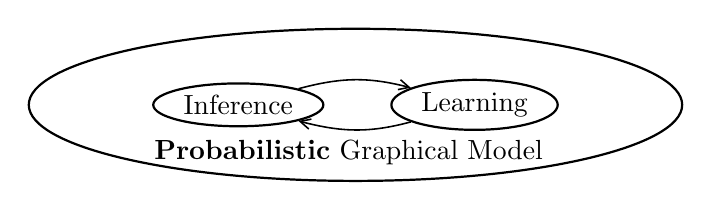
\begin{tikzpicture}
        \tikzstyle{cnode} = [thick, draw=black, ellipse, inner sep = 2pt,  align=center]
        \tikzstyle{fnode} = [thick, draw=black, ellipse, inner sep = 10pt,  align=center]
        
        \node[cnode] (infn) at (0,0) {Inference};
        \node[cnode] (lern) at (3,0) {Learning};
        
        \node[fnode, fit=(infn)(lern)] (box) {};
        \node[] at (1.4, -0.6) {\textbf{Probabilistic} Graphical Model};
        \draw[->,line width=0.2mm] (infn) to[out=15, in=165] (lern);
        \draw[->,line width=0.2mm] (lern) to[out=195, in=-15] (infn);
      \end{tikzpicture}

    \end{figure}
  }

\end{frame}








%%%%%%%%%%%%%%%%%%%%%%%%%%%%%%%%%%%%%%%%%%%%%%%%%%%%%% 
% ------------------------------------------------
%%%%%%%%%%%%%%%%%%%%%%%%%%%%%%%%%%%%%%%%%%%%%%%%%%%%%% 
% \section{Inference}



\subsection{Intuition of Message Passing}
\begin{frame}{What is the state of $x$?}
  \framesubtitle{A toy example}
  Assume that we are interested into the state of node $i$ in an MRF, it can be answered by
  \begin{itemize}[label={$\bullet$}]
  \item the probability $p(x_i)$, or
  \item an empirical version, a collection of samples $\left\{ x_i^n \right\}_{n=1}^{N}$
  \end{itemize}
  It is similar for the case when $\bm{x}$ is of interests, instead of $x_i$.
  \begin{figure}
    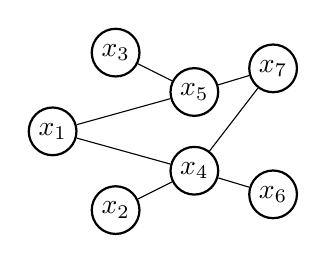
\begin{tikzpicture}
      % \tikzstyle{enode} = [thick, draw=blue, circle, inner sep = 3pt,
      % align=center]
      \tikzstyle{enode} = [thick, draw=black, circle, inner sep = 2pt,  align=center]
      \node[enode] (x1) at (-0.8,0) {$x_1$};
      \node[enode] (x2) at (0,-1) {$x_2$};
      \node[enode] (x3) at (0,1) {$x_3$};
      \node[enode] (x4) at (1,-0.5) {$x_4$};
      \node[enode] (x5) at (1,0.5) {$x_5$};
      \node[enode] (x6) at (2,-0.8) {$x_6$};
      \node[enode] (x7) at (2,+0.8) {$x_7$};

      \draw[-] (x1) to (x4);
      \draw[-] (x1) to (x5);
      \draw[-] (x2) to (x4);
      
      \draw[-] (x3) to (x5);
      \draw[-] (x4) to (x6);
      \draw[-] (x4) to (x7);
      \draw[-] (x5) to (x7);
    \end{tikzpicture}
    \captionsetup{labelformat=empty,justification=centering}
    \caption{what is the state of $x_4$}
    
  \end{figure}
  
\end{frame}

\begin{frame}{What is the state of $x$?}
  \begin{columns}
    \column{0.5\textwidth}
    {Gibbs sampling: let us guess by sampling}
    \vskip 0.5cm
   Sample iteratively: $  x_i \sim p(x_i|\bm{x}_{-i}) \sim p(x_i,\bm{x}_{-i})$
  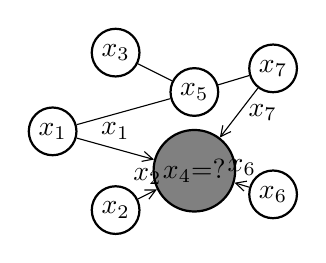
\begin{tikzpicture}
        % \tikzstyle{enode} = [thick, draw=blue, circle, inner sep = 3pt,
        % align=center]
        \tikzstyle{enode} = [thick, draw=black, circle, inner sep = 2pt,  align=center]
        \node[enode] (x1) at (-0.8,0) {$x_1$};
        \node[enode] (x2) at (0,-1) {$x_2$};
        \node[enode] (x3) at (0,1) {$x_3$};
        \node[enode, fill=gray] (x4) at (1,-0.5) {$x_4$=?};
        \node[enode] (x5) at (1,0.5) {$x_5$};
        \node[enode] (x6) at (2,-0.8) {$x_6$};
        \node[enode] (x7) at (2,+0.8) {$x_7$};

        \draw[->] (x1) to node[above] {$x_1$} (x4);
        \draw[-] (x1) to (x5);
        \draw[->] (x2) to node[above] {$x_2$} (x4);
        
        \draw[-] (x3) to (x5);
        \draw[->] (x6) to node[above] {$x_6$} (x4);
        \draw[->] (x7) to node[right] {$x_7$} (x4);
        \draw[-] (x5) to (x7);
      \end{tikzpicture}
      \vskip 0.5cm
      Queries by collected samples $\left\{ \bm{x}^n \right\}_{1}^{N}$.
      
    \column{0.5\textwidth}
    Mean Field and BP: \textit{message in form of sample values $\rightarrow$ message in form of belief}
    \vskip 0.5cm
    Propagating beliefs iteratively
      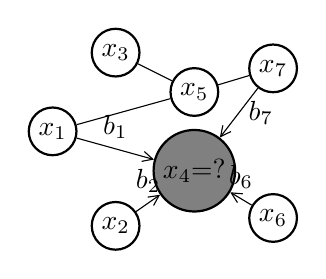
\begin{tikzpicture}
      \tikzstyle{enode} = [thick, draw=black, circle, inner sep = 2pt,  align=center]
      \node[enode] (x1) at (-0.8,0) {$x_1$};
      \node[enode] (x2) at (0,-1.2) {$x_2$};
      \node[enode] (x3) at (0,1) {$x_3$};
      \node[enode, fill=gray] (x4) at (1,-0.5) {$x_4$=?};
      \node[enode] (x5) at (1,0.5) {$x_5$};
      \node[enode] (x6) at (2,-1.1) {$x_6$};
      \node[enode] (x7) at (2,+0.8) {$x_7$};

      \draw[->] (x1) to node[above=0.05mm] {$b_1$} (x4);
      \draw[-] (x1) to (x5);
      \draw[->] (x2) to node[above=0.05mm] {$b_2$}(x4);
      
      \draw[-] (x3) to (x5);
      \draw[->] (x6) to node[above=0.05mm] {$b_6$} (x4);
      \draw[->] (x7) to node[right] {$b_7$} (x4);
      \draw[-] (x5) to (x7);
    \end{tikzpicture}
    \vskip 0.5cm
    Queries by collected samples $\left\{ b_i\right\}$.

    % Corresponding to minimization of \textbf{variational free energy $F_v(b)$  with trial $b$ in fully-factorized form for univariant $\{b_i\}$}.
    \end{columns}
    \let\thefootnote\relax\footnotetext{
      Intuition from \textit{Gibbs (variational) free energy}
        \begin{equation*}
          F_V(b) = \mathrm{KL}(b( \bm{x}) || p(\bm{x}; \bm{\theta})) - \log{Z(\bm{\theta})}
        \end{equation*}
        with trial $b(\bm{x})$. Instance: Bethe free energy.
        }
\end{frame}

% \begin{frame}{What is the state of $x$?}
%   Naive Mean Field: \textbf{message in form of sample values $\rightarrow$ message in form of belief}
%   \begin{figure}
    
%     \begin{tikzpicture}
%       \tikzstyle{enode} = [thick, draw=black, circle, inner sep = 2pt,  align=center]
%       \node[enode] (x1) at (-0.8,0) {$x_1$};
%       \node[enode] (x2) at (0,-1.2) {$x_2$};
%       \node[enode] (x3) at (0,1) {$x_3$};
%       \node[enode, fill=gray] (x4) at (1,-0.5) {$x_4$=?};
%       \node[enode] (x5) at (1,0.5) {$x_5$};
%       \node[enode] (x6) at (2,-1.1) {$x_6$};
%       \node[enode] (x7) at (2,+0.8) {$x_7$};

%       \draw[->] (x1) to node[above=0.05mm] {$b_1$} (x4);
%       \draw[-] (x1) to (x5);
%       \draw[->] (x2) to node[above=0.05mm] {$b_2$}(x4);
      
%       \draw[-] (x3) to (x5);
%       \draw[->] (x6) to node[above=0.05mm] {$b_6$} (x4);
%       \draw[->] (x7) to node[right] {$b_7$} (x4);
%       \draw[-] (x5) to (x7);
%     \end{tikzpicture}
%   \end{figure}
%   Corresponding to minimization of \textbf{variational free energy $F_v(b)$  with trial $b$ in fully-factorized form for univariant $\{b_i\}$}.
%   \let\thefootnote\relax\footnotetext{\tiny
%     Iterative sampling $\rightarrow$ iterative belief update via  
%     \begin{equation*}
%       \log{b_i(x_i)} \propto \sum_{a \in \mathrm{ne}_i} \sum_{\bm{x}_{a} \backslash x_i} \prod_{j\in {a}\backslash i} b_j(x_j)\log{\phi_{a}}(\bm{x}_{a};\bm{\theta}_{a}).
%     \end{equation*}  
%   }
% \end{frame}

% \begin{frame}{What is the state of $x$?}
%   \framesubtitle{Belief propagation (BP): let us guess by propagating belief}
%   \onslide<1->{

%     Proposed by Pearl (1982) for Bayesian networks (tree-structured graphs), which then widely used for general graphs (loopy BP).
    
%     {Yedidia, et al, connected the loopy BP with stationary points of \textbf{Bethe free energy}
%       \begin{align*}
%         F_{Bethe}(b) = \sum_{a\in \Ff} \sum_{\bm{x}_{a}}
%         b_{a}(\bm{x}_{a})\log{\frac{b_{a}(\bm{x}_{a})}{\phi_{a}(\bm{x}_{a})}
%         } -  \sum_{i=1}^{N} (|\mathrm{ne}_i| - 1) \sum_{x_i} b_i(x_i) \log{b_i(x_i)},
%       \end{align*}
%     }
    
%     Corresponding to minimization of approximated \textbf{variational free energy $F_v(b)$  with trial $b$ includes $\{b_i\}$ and $\{b_a\}$}.

%   }
%   \let\thefootnote\relax\footnotetext{\tiny
%     \vskip -0.8cm
%     \begin{align*}
%       \mathrm{msg: factor~ to~ variable} ~~ m_{a\rightarrow i}(x_i) & \propto \sum_{\bm{x}_{a} \backslash x_i}
%                                                                       \phi_{a}(\bm{x}_{a}) \prod_{j \in a \backslash i} m_{j\rightarrow a}(x_j), \\
%       \mathrm{msg: variable~ to~ factor} ~~  m_{j\rightarrow a}(x_j) & \propto  \prod_{a^{\prime} \in \mathrm{ne}_j
%                                                                        \backslash a} m_{a^{\prime}\rightarrow j}(x_j)
%     \end{align*}
%     See, D. Liu, M. T. Vu, Z. Li, and Lars K. Rasmussen. $\alpha$ belief propagation for approximate inference. 2020 \\
%     D. Liu, N. N. Moghadam, L. K. Rasmussen, etc. $\alpha$ belief propagation as fully factorized approximation. In
%     GlobalSIP, 2019.
%     for alternative view to loopy BP.
%   }
  
% \end{frame}



% { \setbeamercolor{background canvas}{bg=hl_bg}
%   \setbeamercolor{normal text}{fg=hl_fg}
%   \setbeamercolor{frametitle}{fg=hl_fg}
%   \begin{frame}
%     \usebeamercolor[fg]{normal text}
%     \begin{center}
%       {\large
%         Play with
%         \textbf{Gibbs (variational) free energy}
%         \begin{equation*}
%           F_V(b) = \mathrm{KL}(b( \bm{x}) || p(\bm{x}; \bm{\theta})) - \log{Z(\bm{\theta})}
%         \end{equation*}
%         with trial $b(\bm{x})$.
%       }
%     \end{center}
    
%   \end{frame}
% }


%%% Local Variables:
%%% mode: latex
%%% TeX-master: "../ppgm_slide"
%%% End:


%%%%%%%%%%%%%%%%%%%%%%%%%%%%%%%%%%%%%%%%%%%%%%%%%%%%%% 
% ------------------------------------------------
% section inference
%%%%%%%%%%%%%%%%%%%%%%%%%%%%%%%%%%%%%%%%%%%%%%%%%%%%%% 

\section{Inference}

{ \setbeamercolor{background canvas}{bg=hl_bg}
  \setbeamercolor{normal text}{fg=hl_fg}
  \setbeamercolor{frametitle}{fg=hl_fg}
  \begin{frame}
    \usebeamercolor[fg]{normal text}
    \begin{center}
      {\large Attempts with neural networks: an imitation game of message passing, or trials under free energy?}
    \end{center}
    
  \end{frame}
}
\subsection{GraphNet}

\begin{frame}{Learn the message update rule by NN}
  An end-to-end learning process: Factor graph $\rightarrow$ converted graph representation $\rightarrow$ GNN $\rightarrow$ Output
  \begin{figure}
    \centerline{\includegraphics[scale=0.3]{images/gnn.png}}
  \end{figure}
  \begin{itemize}[label=$\bullet$]
  \item sum-product update rule (in BP) $\rightarrow$ NN, to learn
  \item pseudo probability (belief aggregation) $\rightarrow$ NN, to learn
  \item end-to-end learning that requires true marginal probability, which BP, GPB and mean field do no require
  \end{itemize}
  \let\thefootnote\relax\footnotetext{\tiny For related methods, see:\\
    Heess et al, Learning to Pass Expectation Propagation Messages\\
    Yoon, et al, 2019, Inference in Probabilistic Graphical Models by Graph Neural Networks\\
    Gilmer, et al, 2017, Neural message passing for quantum chemistry.\\
    Battaglia, et al, 2018, Relational inductive biases, deep learning, and graph networks
  }
\end{frame}

\subsection{AutoEncoder}

% \begin{frame}
%   {Variational Auto-encoder}
%   \onslide<1->{
%     \begin{itemize}[label=$\bullet$]
%     \item Simplification on structures \\
%       \begin{tikzpicture}
%         \tikzstyle{enode} = [thick, draw=black, circle, inner sep = 2pt,  align=center]
%         \tikzstyle{nnode} = [thick, rectangle, rounded corners = 2pt, minimum size = 0.5cm,draw,inner sep = 2pt]
%         \tikzstyle{fnode} = [draw=blue, ellipse, inner sep = 1pt]
%         \tikzstyle{fnoder} = [draw=red, ellipse, inner sep = 0.0pt, rotate=-20]

%         \begin{scope}[scale=0.5]
%           \node[enode] (x1) at (-1.5, 1) {$x_1$};
%           \node[enode] (x2) at (-1.5, -1) {$x_2$};
%           \node[enode] (x3) at (0.5, 1) {$x_3$};
%           \node[enode] (x4) at (0.5, -1) {$x_4$};
%           \draw (x1) -- (x2)
%           (x1) -- (x3)
%           (x4) -- (x3)
%           (x4) -- (x2)
%           ;
%         \end{scope}
%         \begin{scope}[scale=0.5, xshift=5cm]
%           \node[enode] (x1) at (-1.5, 1) {$x_1$};
%           \node[enode] (x2) at (-1.5, -1) {$x_2$};
%           \node[enode] (x3) at (0.5, 1) {$x_3$};
%           \node[enode] (x4) at (0.5, -1) {$x_4$};
%         \end{scope}

%       \end{tikzpicture}
%     }
%     \onslide<2->{
%     \item Care about only a certain set of variables \\
%       \begin{tikzpicture}
%         \tikzstyle{enode} = [thick, draw=black, circle, inner sep = 2pt,  align=center]
%         \tikzstyle{nnode} = [thick, rectangle, rounded corners = 2pt, minimum size = 0.5cm,draw,inner sep = 2pt]
%         \tikzstyle{fnode} = [draw=blue, ellipse, inner sep = 3pt]
        

%         \begin{scope}[scale=0.5]
%           \node[enode] (x1) at (-1.5, 1) {$x_1$};
%           \node[enode] (x2) at (-1.5, -1) {$x_2$};
%           \node[fnode, fit=(x1)(x2)] (xo){$\bm{x}_O$};
%         \end{scope}
%         \begin{scope}[scale=0.5, xshift=5cm]
%           \node[enode] (x3) at (0.5, 1) {$x_3$};
%           \node[enode] (x4) at (0.5, -1) {$x_4$};
%           \node[fnode, fit=(x3)(x4)] (xu) {$\bm{x}_U$};
%         \end{scope}

%       \end{tikzpicture}
%     }
%     \onslide<3->{
%     \item Amortizing the probabilities of interests and learn their parameters by sampling
%       \begin{tikzpicture}
%         \tikzstyle{enode} = [thick, draw=black, circle, inner sep = 2pt,  align=center]
%         \tikzstyle{nnode} = [thick, rectangle, rounded corners = 2pt, minimum size = 0.5cm,draw,inner sep = 2pt]
%         \tikzstyle{fnode} = [draw=blue, ellipse, inner sep = 3pt]
        
%         \node[fnode] (xo) at (0,0){$\bm{x}_O$};
%         \node[fnode] (xu) at (3,0) {$\bm{x}_U$};
%         \node[fnode] (hxo) at (6,0){$\hat{\bm{x}}_O$};
%         \draw[->] (xo) to node[above]{$q(\bm{x}_U|\bm{x}_O)$} (xu);
%         \draw[->](xu) to node[above]{${{p}(\bm{x}_O| \bm{x}_U; \bm{\theta})}$}(hxo);
%       \end{tikzpicture}
      
%       with the \textbf{variational free energy $F_V$ rewritten as}
%       \begin{equation*}
%         F_V(q, \bm{\theta}) = \EE_{q(\bm{x}_U|\bm{x}_O)}\left[ \log{{p}(\bm{x}_O| \bm{x}_U; \bm{\theta})} + \log{{p}(\bm{x}_U; \bm{\theta})} \right] + H({q(\bm{x}_U|\bm{x}_O)}),
%       \end{equation*}
%     }
%   \end{itemize}
% \end{frame}
\subsection{RENN}


\begin{frame}{RENN}
  \framesubtitle{Region revisited}
  \begin{itemize}[label=$\bullet$]
  \item If you cannot collect true targets ($p(x_i)$)
  \item If you are unwilling to be restricted to pre-defined inference  
  \end{itemize}
  \onslide<1->{
    Factor graph representation of MRF (2-by-3 grid) with factor nodes.\\
    MRF $\rightarrow$ region graph:\\
    \begin{columns}
      \column{0.5\textwidth}
      \hskip 1cm
      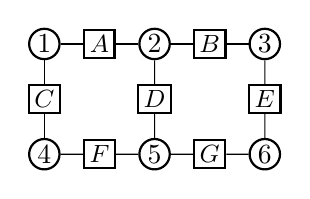
\begin{tikzpicture}
        \begin{scope}[scale=0.7]

          \tikzstyle{cnode} = [thick, draw=black, circle, inner sep = 1pt,  align=center]
          \tikzstyle{nnode} = [thick, rectangle, rounded corners = 0pt,draw,inner sep = 2pt]
          \node[cnode] (x1) at (0,0) {1};
          \node[cnode] (x2) at (2,0) {2};
          \node[cnode] (x3) at (4,0) {3};

          \node[cnode] (x4) at (0,-2) {4};
          \node[cnode] (x5) at (2,-2) {5};
          \node[cnode] (x6) at (4,-2) {6};

          \node[nnode] (fa) at (1,0) {\small$A$};
          \node[nnode] (fb) at (3,0) {\small$B$};

          \node[nnode] (fc) at (0,-1) {\small$C$};
          \node[nnode] (fd) at (2,-1) {\small$D$};
          \node[nnode] (fe) at (4,-1) {\small$E$};
          
          \node[nnode] (ff) at (1,-2) {\small$F$};
          \node[nnode] (fg) at (3,-2) {\small$G$};


          \draw[-] (x1) -- (fa);
          \draw[-] (x1) -- (fc);

          \draw[-] (x2) -- (fa);
          \draw[-] (x2) -- (fb);
          \draw[-] (x2) -- (fd);

          \draw[-] (x3) -- (fb);
          \draw[-] (x3) -- (fe);

          \draw[-] (x4) -- (fc);
          \draw[-] (x4) -- (ff);

          \draw[-] (x5) -- (fd);
          \draw[-] (x5) -- (ff);
          \draw[-] (x5) -- (fg);

          \draw[-] (x6) -- (fe);
          \draw[-] (x6) -- (fg);

        \end{scope}
      \end{tikzpicture}
    }
    \onslide<2->{
      \column{0.5\textwidth}

      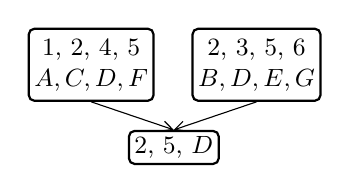
\begin{tikzpicture}
        \tikzstyle{cnode} = [thick, draw=black, circle, inner sep = 1pt,  align=center]
        \tikzstyle{nnode} = [thick, rectangle, rounded corners = 0pt,draw,inner sep = 2pt]

        \begin{scope}[xshift=4.8cm, yshift=-0.3cm,scale=0.7]
          \tikzstyle{rnode} = [thick, rectangle, rounded corners = 2pt,minimum size = 0.0cm,draw,inner sep = 2pt]
          \node[rnode] (r01) at (0,0) {\small \begin{tabular}[x]{@{}c@{}}1, 2, 4, 5 \\ $A,C,D,F$ \end{tabular}};
          \node[rnode] (r02) at (3,0) {\small \begin{tabular}[x]{@{}c@{}}2, 3, 5, 6\\ $B,D,E,G$ \end{tabular}};
          \node[rnode] (r11) at (1.5, -1.5) {\small 2, 5, $D$};

          \draw[->] (r01.south) -- (r11.north);
          \draw[->] (r02.south) -- (r11.north);

        \end{scope}
      \end{tikzpicture}

    \end{columns}
  % }
  % \onslide<3->{
    An alternative region graph of the same MRF:\\
    \centering
    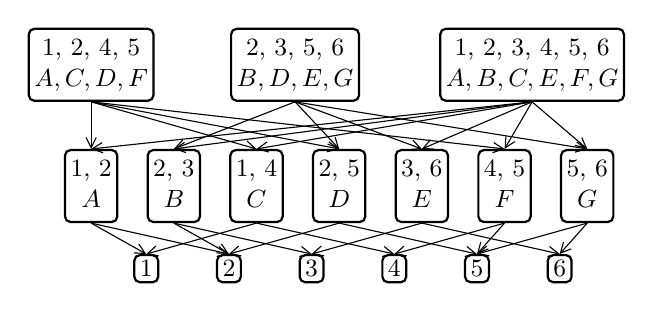
\begin{tikzpicture}
      \tikzstyle{cnode} = [thick, draw=black, circle, inner sep = 1pt,  align=center]
      \tikzstyle{nnode} = [thick, rectangle, rounded corners = 0pt,draw,inner sep = 2pt]

      \begin{scope}[xshift=0.6cm, yshift=-2.35cm,scale=0.7]
        \tikzstyle{rnode} = [thick, rectangle, rounded corners = 2pt,minimum size = 0.0cm,draw,inner sep = 2pt]
        \node[rnode] (r01) at (0,0) {\small\begin{tabular}[x]{@{}c@{}}1, 2, 4, 5 \\ $A,C,D,F$ \end{tabular}};
        \node[rnode] (r02) at (3.7,0) {\small\begin{tabular}[x]{@{}c@{}}2, 3, 5, 6\\ $B,D,E,G$ \end{tabular}};
        \node[rnode] (r03) at (8,0) {\small\begin{tabular}[x]{@{}c@{}}1, 2, 3, 4, 5, 6\\ $A,B,C,E,F,G$ \end{tabular}};
        \begin{scope}[yshift=-0.2cm]
          \node[rnode] (r11) at (0, -2.0) {\small\begin{tabular}[x]{@{}c@{}}1, 2\\ $A$ \end{tabular}};
          \node[rnode] (r12) at (1.5, -2.0) {\small\begin{tabular}[x]{@{}c@{}}2, 3\\ $B$ \end{tabular}};
          \node[rnode] (r13) at (3, -2.0) {\small\begin{tabular}[x]{@{}c@{}}1, 4\\ $C$ \end{tabular}};
          \node[rnode] (r14) at (4.5, -2.0) {\small\begin{tabular}[x]{@{}c@{}}2, 5\\ $D$ \end{tabular}};
          \node[rnode] (r15) at (6, -2.0) {\small\begin{tabular}[x]{@{}c@{}}3, 6\\ $E$ \end{tabular}};
          \node[rnode] (r16) at (7.5, -2.0) {\small\begin{tabular}[x]{@{}c@{}}4, 5\\ $F$ \end{tabular}};
          \node[rnode] (r17) at (9, -2.0) {\small\begin{tabular}[x]{@{}c@{}}5, 6\\ $G$ \end{tabular}};

          \begin{scope}[yshift=0.5cm]
            \node[rnode] (r21) at (1, -4) {\small 1};
            \node[rnode] (r22) at (2.5, -4) {\small 2};
            \node[rnode] (r23) at (4, -4) {\small 3};
            \node[rnode] (r24) at (5.5, -4) {\small 4};
            \node[rnode] (r25) at (7, -4) {\small 5};
            \node[rnode] (r26) at (8.5, -4) {\small 6};
          \end{scope}
        \end{scope}
        % edge level0 to level1
        \draw[->] (r01.south) -- (r11.north);
        \draw[->] (r03.south) -- (r11.north);

        \draw[->] (r02.south) -- (r12.north);
        \draw[->] (r03.south) -- (r12.north);

        \draw[->] (r01.south) -- (r13.north);
        \draw[->] (r03.south) -- (r13.north);

        \draw[->] (r01.south) -- (r14.north);
        \draw[->] (r02.south) -- (r14.north);

        \draw[->] (r02.south) -- (r15.north);
        \draw[->] (r03.south) -- (r15.north);

        \draw[->] (r01.south) -- (r16.north);
        \draw[->] (r03.south) -- (r16.north);

        \draw[->] (r02.south) -- (r17.north);
        \draw[->] (r03.south) -- (r17.north);

        % edge level1 to level2
        \draw[->] (r11.south) -- (r21.north);
        \draw[->] (r13.south) -- (r21.north);

        \draw[->] (r11.south) -- (r22.north);
        \draw[->] (r12.south) -- (r22.north);
        \draw[->] (r14.south) -- (r22.north);


        \draw[->] (r12.south) -- (r23.north);
        \draw[->] (r15.south) -- (r23.north);

        \draw[->] (r13.south) -- (r24.north);
        \draw[->] (r16.south) -- (r24.north);

        \draw[->] (r14.south) -- (r25.north);
        \draw[->] (r16.south) -- (r25.north);
        \draw[->] (r17.south) -- (r25.north);

        \draw[->] (r15.south) -- (r26.north);
        \draw[->] (r17.south) -- (r26.north);
      \end{scope}
    \end{tikzpicture}
  }
\end{frame}
\begin{frame}{RENN}
  \onslide<1->{
    The region-based free energy of a region graph is
    \begin{equation*}
      F_R(\Bb; \bm{\theta}) = \sum_{R\in \Rr} \underbrace{c_R}_{counting~number} \sum_{\bm{x}_R}b_R(\bm{x}_R) (\underbrace{E_R(\bm{x}_R; \bm{\theta}_R)}_{region~average~energy} + \ln{b_R}(\bm{x}_R)),
    \end{equation*}
    \begin{itemize}[label=$\bullet$]
    \item counting number: balance the contribution of each region
    \item region average energy: $- \sum_{a\in A_R} \ln{\phi_a(\bm{x}_a; \bm{\theta}_a)}$
    \end{itemize}
  }
  \onslide<2->{
    \begin{columns}
      \column{0.05\textwidth}
      Denote
      \column{0.3\textwidth}
      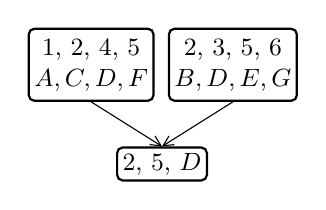
\begin{tikzpicture}
        \tikzstyle{cnode} = [thick, draw=black, circle, inner sep = 1pt,  align=center]
        \tikzstyle{nnode} = [thick, rectangle, rounded corners = 0pt,draw,inner sep = 2pt]
        
        \begin{scope}[xshift=0cm, yshift=-2.3cm,scale=0.6]
          \tikzstyle{rnode} = [thick, rectangle, rounded corners = 2pt,minimum size = 0.0cm,draw,inner sep = 2pt]
          \node[rnode] (r01) at (0,0) {\small \begin{tabular}[x]{@{}c@{}}1, 2, 4, 5 \\ $A,C,D,F$ \end{tabular}};
          \node[rnode] (r02) at (3,0) {\small \begin{tabular}[x]{@{}c@{}}2, 3, 5, 6\\ $B,D,E,G$ \end{tabular}};
          \node[rnode] (r11) at (1.5, -2.1) {\small 2, 5, $D$};

          \draw[->] (r01.south) -- (r11.north);
          \draw[->] (r02.south) -- (r11.north);

        \end{scope}
      \end{tikzpicture}
      \column{0.05\textwidth}
      by
      \column{0.3\textwidth}

      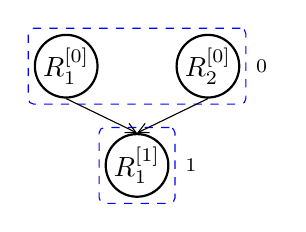
\begin{tikzpicture}
        \tikzstyle{cnode} = [thick, draw=black, circle, inner sep = 1pt,  align=center]
        \tikzstyle{nnode} = [dashed, draw=blue, rectangle, rounded corners = 2pt, inner sep = 2pt]
        
        \begin{scope}[xshift=0cm, yshift=2.3cm,scale=0.6]
          \tikzstyle{rnode} = [thick, circle, rounded corners = 2pt,minimum size = 0.0cm,draw,inner sep = 0.5pt]
          \node[rnode] (r01) at (0,0) {$R_1^{[0]}$};
          \node[rnode] (r02) at (3,0) {$R_2^{[0]}$};
          \node[rnode] (r11) at (1.5, -2.1) {$R_1^{[1]}$};
          \node[nnode, fit=(r01)(r02), label=right:$\Rr_0$] {};
          \node[nnode, fit=(r11), label=right:$\Rr_1$] {};

          \draw[->] (r01.south) -- (r11.north);
          \draw[->] (r02.south) -- (r11.north);

        \end{scope}
      \end{tikzpicture}
    \end{columns}
  }
  \onslide<3->{
    \begin{columns}
      \column{0.1\textwidth}
      Amortizing root beliefs:
      \column{0.7\textwidth}

      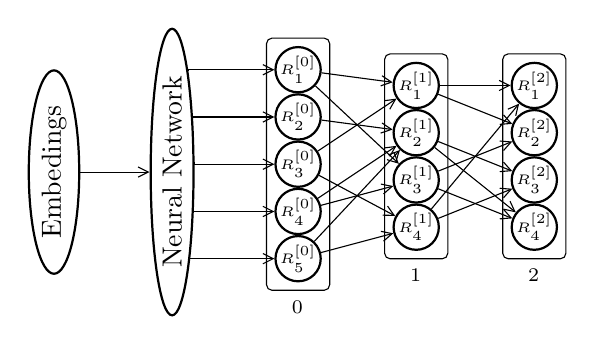
\begin{tikzpicture}
        
        \tikzstyle{enode} = [thick, draw=black, ellipse, inner sep = 2pt,  align=center]
        \tikzstyle{cnode} = [thick, draw=black, circle, inner sep = 0.0pt,  align=center]
        \tikzstyle{nnode} = [thick, rectangle, rounded corners = 0pt,draw,inner sep = 2pt]
        \begin{scope}[xshift=-1cm, yshift=-1.3cm, scale=0.6]
          \node[enode, rotate=90] (em) at (-2.5,0) {Embedings};
          \node[enode, rotate=90] (nn) {Neural Network};
        \end{scope}
        
        % level0 regions
        \begin{scope}[scale=0.6]
          \node[cnode] (r01) at (1, 0) {\tiny$R_1^{[0]}$};
          \node[cnode] (r02) at (1, -1) {\tiny$R_2^{[0]}$};
          \node[cnode] (r03) at (1, -2) {\tiny$R_3^{[0]}$};
          \node[cnode] (r04) at (1, -3) {\tiny$R_4^{[0]}$};
          \node[cnode] (r05) at (1, -4) {\tiny$R_5^{[0]}$};
          \node[label=below:$\Rr_0$, draw,rounded corners = 2pt, inner sep=1mm, fit=(r01) (r05)] {};
        \end{scope}

        \draw[->] (nn.351.9) |- (r01);
        \draw[->] (nn.340) |- (r02);
        \draw[->] (nn.295) |- (r03);
        \draw[->] (nn.210) |- (r04);
        \draw[->] (nn.191) |- (r05);

        \draw[->] (em) -- (nn);


        % level 1 regions
        \begin{scope}[xshift=1.5cm, yshift=-0.2cm, scale=0.6]
          \node[cnode] (r11) at (1, 0) {\tiny$R_1^{[1]}$};
          \node[cnode] (r12) at (1, -1) {\tiny$R_2^{[1]}$};
          \node[cnode] (r13) at (1, -2) {\tiny$R_3^{[1]}$};
          \node[cnode] (r14) at (1, -3) {\tiny$R_4^{[1]}$};
          \node[label=below:$\Rr_1$, draw, rounded corners = 2pt, inner sep=1mm, fit=(r11) (r14)] {};
        \end{scope}

        
        
        % level 1 regions
        \begin{scope}[xshift=3cm, yshift=-0.2cm, scale=0.6]
          \node[cnode] (r21) at (1, 0) {\tiny$R_1^{[2]}$};
          \node[cnode] (r22) at (1, -1) {\tiny$R_2^{[2]}$};
          \node[cnode] (r23) at (1, -2) {\tiny$R_3^{[2]}$};
          \node[cnode] (r24) at (1, -3) {\tiny$R_4^{[2]}$};
          \node[label=below:$\Rr_2$, draw, rounded corners = 2pt, inner sep=1mm, fit=(r21) (r24)] {};
        \end{scope}

        \draw[->] (r01) -- (r11);
        \draw[->] (r03) -- (r11);

        \draw[->] (r02) -- (r12);
        \draw[->] (r04) -- (r12);
        \draw[->] (r05) -- (r12);

        \draw[->] (r01) -- (r13);
        \draw[->] (r04) -- (r13);

        \draw[->] (r03) -- (r14);
        \draw[->] (r05) -- (r14);


        \draw[->] (r11) -- (r21);
        \draw[->] (r14) -- (r21);

        \draw[->] (r11) -- (r22);
        \draw[->] (r13) -- (r22);

        \draw[->] (r12) -- (r23);
        \draw[->] (r14) -- (r23);

        \draw[->] (r12) -- (r24);
        \draw[->] (r13) -- (r24);

        
        
      \end{tikzpicture}
    \end{columns}
  }
\end{frame}

\begin{frame}{RENN}
  \onslide<1->{
    Objective of RENN\footnote{\tiny More detail on RENN? Refer to, Dong Liu, Ragnar Thobaben, and Lars K. Rasmussen. Region-based energy
      neural network for approximate inference. arxiv, 2020}:\\
    \begin{equation*}
      \min \mathrm{\textbf{region-based free energy}} (F_R) + \underbrace{\mathrm{\textbf{panelty on belief consistency} }}_{along~ region~ graph~ struture}
    \end{equation*}
  }
  \\
  \onslide<2->{
    Inference only\\
    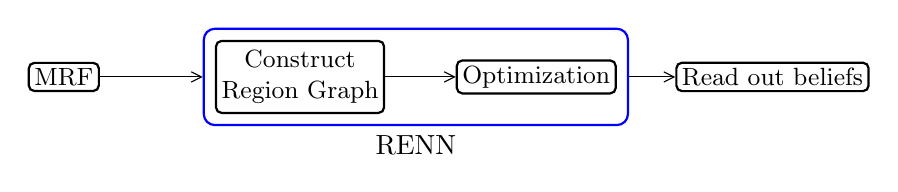
\begin{tikzpicture}
      \tikzstyle{cnode} = [thick, draw=blue, rounded corners = 4pt, rectangle, inner sep = 4pt,  align=center]
      \tikzstyle{nnode} = [thick, rectangle, rounded corners = 0pt,draw,inner sep = 2pt]
      \tikzstyle{rnode} = [thick, rectangle, rounded corners = 2pt,minimum size = 0.0cm,draw,inner sep = 2pt]
      
      \node[rnode] (r01) at (-1,0) {\small MRF};
      \node[rnode] (r02) at (2,0) {\small \begin{tabular}[x]{@{}c@{}} Construct\\ Region Graph \end{tabular}};
      \node[rnode] (r03) at (5, 0) {\small Optimization};
      \node[rnode] (r04) at (8, 0) {\small Read out beliefs};
      \node[cnode, fit=(r02)(r03), label=below:{RENN}] (renn) {};

      \draw[->] (r01) -- (renn);
      \draw[->] (renn) -- (r04);
      \draw[->] (r02) -- (r03);
    \end{tikzpicture}
  }
  \onslide<3->{
    Learning alternatives of MRFs
    \vskip 0.2cm
    \begin{columns}
      \column{0.5\textwidth}
      learn with customized optm.
      \begin{align*}
        \pd{\log{p}(\bm{x};\bm{\theta})}{\bm{\theta}_a} = &\pd{\log{{\phi_a}(\bm{x}_a; \bm{\theta}_a)}}{\bm{\theta}_a} \\
                                                          &- \underbrace{\EE_{p(\bm{x}_a; \bm{\theta})}\left[ \pd{\log{{\phi_a}(\bm{x}_a; \bm{\theta}_a)}}{\bm{\theta}_a} \right]}_{est.~ beliefs}.
      \end{align*}
    }
    \onslide<4->{
      \column{0.5\textwidth}
      learn with auto-grads
      \begin{align*}
        \max_{\bm{\theta}} \log{p(\bm{x}; \bm{\theta})} =  \max_{\bm{\theta}}&\sum_{a}\log{ \psi_a(\bm{x}_a; \bm{\theta}_a) } \\
                                                                             &-\underbrace{ \log{Z(\bm{\theta})}}_{ets.~ free~energy},
      \end{align*}
      by $-\log{Z(\bm{\theta})} \simeq F_R$.

    \end{columns}
  }
  
\end{frame}

% \section{Some Numerical Evaluation}
\subsection{Numericals}
\begin{frame}
  {Inference results}
  Ising model: $p(\bm{x}; \bm{\theta}) = \frac{1}{Z(\bm{\theta})}\exp{(\sum_{(i,j)\in \Ee_F} J_{ij} x_i x_j + \sum_{i\in \Vv}h_i x_i)}$, $\bm{x} \in \{-1, 1\}^{N}$,
  \begin{itemize}[label=$\bullet$]
  \item $J_{ij}$ is the pairwise log-potential between node $i$ and $j$, $J_{ij}\sim \Nn(0,1)$
  \item  $h_i$ is the node log-potential for node $i$, $h_i \sim \Nn(0, \gamma^{2})$
  \end{itemize}
  
  Inference on grid graph ($\gamma=0.1$). 
  \begin{adjustbox}{width=1\textwidth}
    \begin{tabular}{lcccccccc}
      \toprule
      Metric & $n$ & Mean Field & Loopy BP & Damped BP & GBP & Inference Net & RENN \\
      \midrule
      \multirow{4}{*}{\begin{tabular}[x]{@{}c@{}}$\ell_1$\\error \end{tabular} }
             &    25   &$0.271 \pm 0.051$ &  $0.086 \pm 0.078$ & $0.084 \pm 0.076$ & $0.057 \pm 0.024$ & $0.111 \pm 0.072$ & \textbf{0.049} $\pm$ 0.078 \\

             &    100   & $0.283 \pm 0.024$ &  $0.085 \pm 0.041$ & $0.062 \pm 0.024$ & $0.064 \pm 0.019$ & $0.074 \pm 0.034$ & \textbf{0.025} $\pm$ 0.011 \\

             &    225   & $0.284 \pm 0.019$ &  $0.100 \pm 0.025$ & $0.076 \pm 0.025$ & $0.073 \pm 0.013$ & $ 0.073 \pm 0.012$ & \textbf{0.046} $\pm$ 0.011 \\

             &    400   & $0.279 \pm 0.014$ &  $0.110 \pm 0.016$ & $0.090 \pm 0.016$ & $0.079 \pm 0.009$ & $ 0.083 \pm 0.009$ & \textbf{0.061} $\pm$ 0.009 \\

      \midrule
      \multirow{4}{*}{\begin{tabular}[x]{@{}c@{}}Corre-\\lation\\ $\rho$ \end{tabular}}
             &   25    & 0.633 $\pm$ 0.197  &  0.903 $\pm$ 0.114  &  0.905 $\pm$ 0.113  &  0.923 $\pm$ 0.045  &  0.866$\pm$ 0.117 &  \textbf{0.951} $\pm$ 0.112 \\

             &   100   & 0.582 $\pm$ 0.112  &  0.827 $\pm$ 0.134  &  0.902 $\pm$ 0.059  &  0.899 $\pm$ 0.043  &  0.903$\pm$ 0.049 &   \textbf{0.983} $\pm$ 0.012 \\

             &   225   & 0.580 $\pm$ 0.080  &  0.801 $\pm$ 0.078  &  0.863 $\pm$ 0.088  &  0.869 $\pm$ 0.037  & 0.873 $\pm$ 0.037 &  \textbf{0.949} $\pm$ 0.022 \\

             &   400   & 0.596 $\pm$ 0.054  &  0.779 $\pm$ 0.059  &  0.822 $\pm$ 0.047  &  0.852 $\pm$ 0.024  & 0.841 $\pm$ 0.028 &  \textbf{0.912} $\pm$ 0.025 \\

      \midrule
      \multirow{4}{*}{\begin{tabular}[x]{@{}c@{}}$\log{Z}$ \\error\end{tabular}}
             &   25    & 2.512 $\pm$ 1.060  &  0.549 $\pm$ 0.373  &  0.557 $\pm$ 0.369  &  \textbf{0.169} $\pm$ 0.142  &  0.762 $\pm$ 0.439  &  0.240 $\pm$ 0.140 \\

             &  100    & 13.09 $\pm$ 2.156  &  1.650 $\pm$ 1.414  &  1.457 $\pm$  1.365 &  \textbf{0.524} $\pm$ 0.313  &  2.836 $\pm$ 2.158  & 1.899 $\pm$ 0.495 \\

             &  225    & 29.93 $\pm$ 4.679  &  3.348 $\pm$ 1.954  &  3.423 $\pm$ 2.157  &  \textbf{1.008} $\pm$ 0.653  &  3.249 $\pm$ 2.058  & 4.344 $\pm$ 0.813  \\

             &  400    & 51.81 $\pm$ 4.706  &  5.738 $\pm$ 2.107  &  5.873$\pm$ 2.211   &  \textbf{1.750} $\pm$ 0.869  &  3.953 $\pm$ 2.558  & 7.598 $\pm$ 1.146 \\

      \bottomrule
    \end{tabular}
  \end{adjustbox}
  \begin{itemize}[label=$\bullet$]
  \item $\ell_1$ error of beliefs v.s. true
  \item correlation $\rho$ between true and approximate marginals,
  \item $\log{Z}$ error, true v.s. free energy approximation.
  \end{itemize}


  % \begin{table*}
  %   \caption{Inference on grid Graph. ($\gamma=1$)}
  %   \label{apdx:table:infer-grid-gamma1.0}
  %   \vskip -0.1in
  %   \begin{adjustbox}{width=1\textwidth}
  %     \begin{tabular}{lcccccccc}
  %       \toprule
  %       Metric & $n$ & Mean Field & Loopy BP & Damped BP & GBP & Inference Net & RENN \\
  %       \midrule
  %       \multirow{4}{*}{\begin{tabular}[x]{@{}c@{}}$\ell_1$\\error \end{tabular} }
  %       & 25   &  0.131 $\pm$ 0.080  &  \textbf{0.022} $\pm$ 0.017  &  0.022 $\pm$ 0.018  &  0.137 $\pm$ 0.026  &  0.043 $\pm$ 0.017  &  0.027 $\pm$ 0.014 \\
  %       & 100  &  0.130 $\pm$ 0.041  &  0.025 $\pm$ 0.014  &  0.025 $\pm$ 0.014  &  0.146 $\pm$ 0.020  &  0.046 $\pm$ 0.009  &  \textbf{0.017} $\pm$ 0.002  \\

  %       &225   &  0.135 $\pm$ 0.024  &  0.024 $\pm$ 0.010  &  0.023 $\pm$ 0.009  &  0.154 $\pm$ 0.012  &  0.052 $\pm$ 0.010  &  \textbf{0.017} $\pm$ 0.003 \\

  %       &400   &  0.131 $\pm$ 0.020  &  0.020 $\pm$ 0.003  &  0.020 $\pm$ 0.003  &  0.158 $\pm$ 0.007  &  0.052 $\pm$ 0.007  &  \textbf{0.017} $\pm$ 0.001  \\



  %       \midrule
  %       \multirow{4}{*}{\begin{tabular}[x]{@{}c@{}}Corre-\\lation \\$\rho$\end{tabular}}
  %       & 25   &  0.849 $\pm$ 0.159  &  \textbf{0.992} $\pm$ 0.011  &  0.991 $\pm$ 0.012  &  0.798 $\pm$ 0.088  &  0.980 $\pm$ 0.015  & 0.988 $\pm$ 0.025  \\
  %       & 100  &  0.841 $\pm$ 0.087  &  0.988 $\pm$ 0.013  &  0.988 $\pm$ 0.012  &  0.788 $\pm$ 0.051  &  0.976 $\pm$ 0.013  &  \textbf{0.997} $\pm$0.001 \\

  %       & 225  &  0.824 $\pm$ 0.057  &  0.989 $\pm$ 0.010  &  0.990 $\pm$ 0.010  &  0.764 $\pm$ 0.022  &  0.966 $\pm$ 0.016  &  \textbf{0.996} $\pm$ 0.001 \\

  %       & 400  &  0.828 $\pm$ 0.043  &  0.993 $\pm$ 0.002  &  0.993 $\pm$ 0.002  &  0.759 $\pm$ 0.018  &  0.967 $\pm$ 0.013  &  \textbf{0.997} $\pm$ 0.001  \\

  %       \midrule
  %       \multirow{4}{*}{\begin{tabular}[x]{@{}c@{}}$\log{Z}$ \\error\end{tabular}}
  %       & 25  &  2.113 $\pm$ 1.367  &  \textbf{0.170} $\pm$ 0.199  &  0.194 $\pm$ 0.188  &  0.605 $\pm$ 0.611  &  2.214 $\pm$ 0.775  &  0.649 $\pm$ 0.363  \\

  %       &100  &  8.034 $\pm$ 2.523  &  \textbf{0.372} $\pm$ 0.427  &  0.415 $\pm$ 0.422  &  1.545 $\pm$ 1.081  &  11.14 $\pm$ 0.954  &  3.129 $\pm$ 0.520  \\

  %       &225  &  17.923 $\pm$ 3.474 &  0.952 $\pm$ 1.037  &  \textbf{0.917} $\pm$ 0.922  &  3.143 $\pm$ 2.122  &  25.55 $\pm$ 2.025  &  7.473 $\pm$ 0.906  \\

  %       &400  &  31.74 $\pm$ 4.766          &  \textbf{0.919} $\pm$ 0.684   &  1.011 $\pm$ 0.685  &  3.313 $\pm$ 1.872  &  46.61 $\pm$ 3.094  &  12.77 $\pm$ 0.991  \\

  %       \bottomrule
  %     \end{tabular}
  %   \end{adjustbox}
  % \end{table*}
  \let\thefootnote\relax\footnotetext{\tiny
    Inference Net: Wiseman, Kim, Amortized Bethe Free Energy Minimization for Learning MRFs, 2019.
  }
\end{frame}
\begin{frame}
  {Learning MRFs}
  What is $\bm{\theta}$ in $p(\bm{x};\bm{\theta})$?\\
  Table of negative log-likelihood of learned MRFs \\
  \begin{adjustbox}{width=1\textwidth}
    \begin{tabular}{lcccccccc}
      % std=1.0
      \toprule
      $n$ & True & Exact & Mean Field & Loopy BP & Damped BP & GBP & Inference Net & RENN \\
      \toprule
      \multicolumn{9}{c}{Grid Graph}\\
      \midrule
      25  &  9.000  &  9.004  &  9.811  &  {9.139}  &  9.196  &  10.56  &  9.252  &  \textbf{9.048}  \\
      100 &  19.34  &  19.38  &  23.48  &  {19.92}  &  20.02  &  28.61  &  20. 29  &  \textbf{19.76} \\
      225 &  63.90  &  63.97  &  69.01  &  66.44    &  66.25  &  92.62  &  68.15  &  \textbf{64.79}  \\
      \toprule
      % std=1.0
      \multicolumn{9}{c}{Complete Graph}\\
      \midrule
      9  &  3.276  &  3.286  &  9.558  &  5.201  &  5.880  &  10.06  &  5.262  & \textbf{3.414}  \\
      16  &  4.883  &  4.934  &  28.74  &  13.64  &  18.95  &  24.45  &  13.77  &  \textbf{5.178}  \\

      \bottomrule
    \end{tabular}
  \end{adjustbox}
\end{frame}

%%% Local Variables:
%%% mode: latex
%%% TeX-master: "../ppgm_slide"
%%% End:



%%%%%%%%%%%%%%%%%%%%%%%%%%%%%%%%%%%%%%%%%%%%%%%%%%%%%% 
% ------------------------------------------------
% section learning
%%%%%%%%%%%%%%%%%%%%%%%%%%%%%%%%%%%%%%%%%%%%%%%%%%%%%% 
\section{Learning}
\subsection{Bidirectional Impact}

{ \setbeamercolor{background canvas}{bg=hl_bg}
  \setbeamercolor{normal text}{fg=hl_fg}
  \setbeamercolor{frametitle}{fg=hl_fg}
  \begin{frame}
    \usebeamercolor[fg]{normal text}
    \begin{center}
      {
        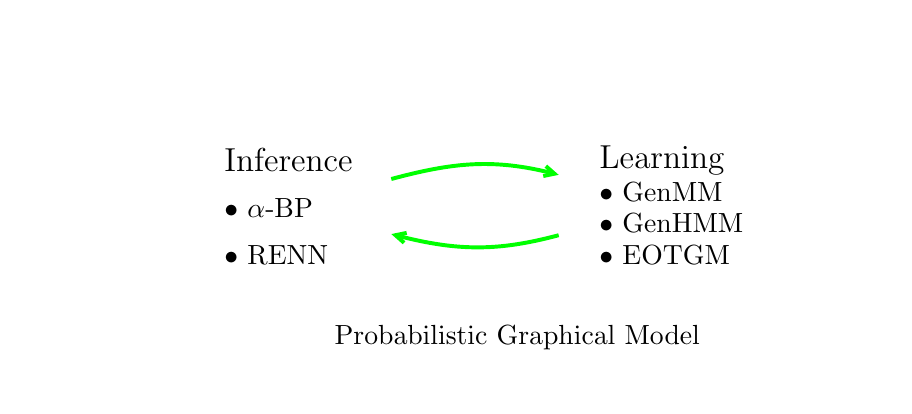
\begin{tikzpicture}
          \tikzstyle{cnode} = [thick, draw=white, ellipse, inner sep = 2pt,  align=center]
          \tikzstyle{fnode} = [thick, draw=white, ellipse, inner sep = 10pt,  align=center]
          \tikzstyle{rnode} = [thick, rectangle, inner sep = 1.5pt,  align=left]
          \node[rnode] (inf) at (-2, 0) {\large Inference};
          \node[rnode, below = 0.6cm of inf.west, anchor=west] (abp) {$\bullet$ {$\alpha$-BP}};
          \node[rnode, below = 1.2cm of inf.west, anchor=west] (renn) {$\bullet$ RENN};
          \node[cnode, fit=(abp)(inf)(renn)] (infn) {};
          
          \node[rnode, right = 3 of inf] (lern) {\large Learning};
          \node[rnode, below = 0.4 of lern.west, anchor=west] (genmm) {$\bullet$ GenMM};
          \node[rnode, below = 0.8 of lern.west, anchor=west] (genhmm) {{$\bullet$} GenHMM};
          \node[rnode, below = 1.2 of lern.west, anchor=west] (lfree) {{$\bullet$} EOTGM};
          \node[cnode, fit=(lern)(genmm)(genhmm)(lfree)] (learn) {};

          \node[fnode, fit=(infn)(lern)] (box) {};

          
          \node[below right = 0.5 and -0.5 of infn] {{Probabilistic} Graphical Model};
          \draw[->,line width=0.5mm, green] (infn) to[out=15, in=165] (learn);
          \draw[->,line width=0.5mm, green] (learn) to[out=195, in=-15] (infn);
        \end{tikzpicture}
      }
    \end{center}
    
  \end{frame}
}
\begin{frame}{Two Direction Impact}
  Why impact in two direction?
  \begin{itemize}[label=$\bullet$]
    
    \item Learning to Inference:\\
      \begin{figure}[!t]
        \centering
        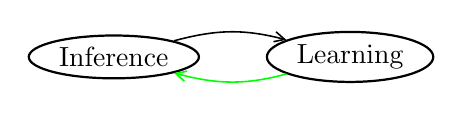
\begin{tikzpicture}
          \tikzstyle{cnode} = [thick, draw=black, ellipse, inner sep = 2pt,  align=center]
          \tikzstyle{fnode} = [thick, draw=black, ellipse, inner sep = 10pt,  align=center]
          
          \node[cnode] (infn) at (0,0) {Inference};
          \node[cnode] (lern) at (3,0) {Learning};
          
          % \node[fnode, fit=(infn)(lern)] (box) {};
          % \node[] at (1.4, -0.6) {Probabilistic Graphical Model};
          \draw[->,line width=0.2mm] (infn) to[out=15, in=165] (lern);
          \draw[green, ->,line width=0.2mm] (lern) to[out=195, in=-15] (infn);
        \end{tikzpicture}
      \end{figure}
      Stuff we have been taken as default, a given $p(\bm{x};\bm{\theta})$
      \begin{itemize}[label=$\bullet$]
      \item built by expert knowledge, or
      \item built by extracting information from evidence (empirical data).
      \end{itemize}
    \item Inference to Learning:\\
      \begin{figure}[!t]
        \centering
        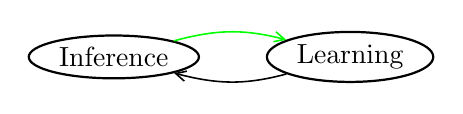
\begin{tikzpicture}
          \tikzstyle{cnode} = [thick, draw=black, ellipse, inner sep = 2pt,  align=center]
          \tikzstyle{fnode} = [thick, draw=black, ellipse, inner sep = 10pt,  align=center]
          
          \node[cnode] (infn) at (0,0) {Inference};
          \node[cnode] (lern) at (3,0) {Learning};
          
          % \node[fnode, fit=(infn)(lern)] (box) {};
          % \node[] at (1.4, -0.6) {Probabilistic Graphical Model};
          \draw[green, ->,line width=0.2mm] (infn) to[out=15, in=165] (lern);
          \draw[->,line width=0.2mm] (lern) to[out=195, in=-15] (infn);
        \end{tikzpicture}
      \end{figure}
      Model learning: an error trial process that compares inferred 'fact' and actual fact (evidence).\\
      Model learning usually needs inference as a subroutine, which sometimes are replaced by sampling in particle based methods.
    
  \end{itemize}
  
  
\end{frame}
\begin{frame}{\large Inference Routine in Learning}
  
  What is $\bm{\theta}$ in $p(\bm{x}; \bm{\theta}) = \frac{1}{Z(\bm{\theta})} \prod_{a} \psi_a(\bm{x}_a; \bm{\theta}_a)$? \\
  A direct view:
  \begin{align*}
    \max_{\bm{\theta}} \log{p(\bm{x}; \bm{\theta})} =  \max_{\bm{\theta}}\sum_{a}\log{ \psi_a(\bm{x}_a; \bm{\theta}_a) } \underbrace{- \log{Z(\bm{\theta})}}_{\text{Helmholtz free energy, can be est. by $F$}},
  \end{align*}
  An alternative view:
  \begin{align*}
    \pd{\log{p}(\bm{x};\bm{\theta})}{\bm{\theta}_a} = \pd{\log{{\phi_a}(\bm{x}_a; \bm{\theta}_a)}}{\bm{\theta}_a} - \underbrace{\EE_{p(\bm{x}_a; \bm{\theta})}\left[ \pd{\log{{\phi_a}(\bm{x}_a; \bm{\theta}_a)}}{\bm{\theta}_a} \right]}_{\text{can be est. by beliefs}}.
  \end{align*}

  Remark:
  \begin{itemize}[label={$\bullet$}]
  \item This essentially requires estimation of Helmholtz free energy or marginal probabilities.
  \item Stationary points translate into moment matching.
  \end{itemize}
  \only<2->{
  \begin{textblock}{5}(3,10)
    \begin{tikzpicture}[auto,rotate=-5,transform shape]
      \tikzstyle{cnode} = [thick, draw=black, ellipse, inner sep = 2pt,  align=center]
      \tikzstyle{fnode} = [thick, draw=black, ellipse, inner sep = 10pt,  align=center]
          
      \node[cnode] (infn) at (0,0) {Inference};
      \node[cnode] (lern) at (3,0) {Learning};
      
      \draw[->,line width=0.2mm] (infn) to[out=15, in=165] (lern);
      \draw[->,line width=0.2mm] (lern) to[out=195, in=-15] (infn);

      \node[text width=7cm, align=left, below =of infn.west, anchor=west] (uncouple)
      {\begin{minipage}{1\textwidth}
          \begin{itemize}[label=\textbullet]
          \item Two modules are not necessarily coupled
          \item Each module may be replaced by another algorithm while the other one remains.
          \end{itemize}
        \end{minipage}
      };
      \begin{scope}[on background layer]
        \node [rounded corners = 4pt, rectangle, inner sep = 4pt,  align=center, fit=(uncouple)(infn)(lern), label=below:{}, fill=\stampcolor] () {};
      \end{scope}
    \end{tikzpicture}
  \end{textblock}
}
\end{frame}

% \begin{frame}[label=current]{\large Inference Routine in Learning}
%   \begin{tikzpicture}
%     \node[black] (grad) at (0,0) {
%     \begin{minipage}{1\linewidth}
%       What is $\bm{\theta}$ in $p(\bm{x}; \bm{\theta}) = \frac{1}{Z(\bm{\theta})} \prod_{a} \psi_a(\bm{x}_a; \bm{\theta}_a)$? \\
%       A direct view:
%       \begin{align*}
          %           \max_{\bm{\theta}} \log{p(\bm{x}; \bm{\theta})} =  \max_{\bm{\theta}}\sum_{a}\log{ \psi_a(\bm{x}_a; \bm{\theta}_a) } \underbrace{- \log{Z(\bm{\theta})}}_{\text{Helmholtz free energy, can be est. by $F$}},
          %         \end{align*}
          %           An alternative view:
          %           \begin{align*}
          %           \pd{\log{p}(\bm{x};\bm{\theta})}{\bm{\theta}_a} = \pd{\log{{\phi_a}(\bm{x}_a; \bm{\theta}_a)}}{\bm{\theta}_a} - \underbrace{\EE_{p(\bm{x}_a; \bm{\theta})}\left[ \pd{\log{{\phi_a}(\bm{x}_a; \bm{\theta}_a)}}{\bm{\theta}_a} \right]}_{\text{can be est. by beliefs}}.
          %         \end{align*}

          %           Remark:
          %           \begin{itemize}[label={$\bullet$}]
          %           \item This essentially requires estimation of Helmholtz free energy or marginal probabilities.
          %           \item Stationary points translate into moment matching.
          %           \end{itemize}
          %           \end{minipage}
          %           };
          %           \pause {
          %           \begin{scope}[local bounding box=uncouple]
          %           \tikzstyle{cnode} = [thick, draw=black, ellipse, inner sep = 2pt,  align=center]
          %           \tikzstyle{fnode} = [thick, draw=black, ellipse, inner sep = 10pt,  align=center]

          %           \node[cnode] (infn) at (0,0) {Inference};
          %           \node[cnode] (lern) at (3,0) {Learning};
          %           \node[black, above=of infn.north] (txt1) {at The two modules are not necessarily coupled};
          %         %           \node[fnode, fit=(infn)(lern)] (box) {};
          %         %           \node[] at (1.4, -0.6) {Probabilistic Graphical Model};
          %           \draw[->,line width=0.2mm] (infn) to[out=15, in=165] (lern);
          %           \draw[->,line width=0.2mm] (lern) to[out=195, in=-15] (infn);
          %           \node[black,fill=white, below=of infn.south] (txt2) {Each module may be replaced by another algorithm while the other one remains.};
          %           \begin{scope}[on background layer]
          %           \node[rectangle, inner sep = 10pt,  align=center, fit=(txt1)(txt2)(infn)(learn), fill=white] {};
          %           \end{scope}

          %           \end{scope}

          %           }  
          %           \end{tikzpicture}
          %           \end{frame}




\begin{frame}
  {Learning MRFs}
  {What is $\bm{\theta}$ in $p(\bm{x};\bm{\theta})$?}
  \vskip 0.5cm
  Table of negative log-likelihood of learned MRFs \\
  \begin{table}
    \begin{adjustbox}{width=0.9\textwidth}
      \begin{tabular}{lcccccccc}
        % std=1.0
        \toprule
        N & True & Exact & Mean Field & Loopy BP & Damped BP & GBP & Inference Net & RENN \\
        \toprule
        \multicolumn{9}{c}{Grid Graph}\\
        \midrule
        25  &  9.000  &  9.004  &  9.811  &  {9.139}  &  9.196  &  10.56  &  9.252  &  \textbf{9.048}  \\
        100 &  19.34  &  19.38  &  23.48  &  {19.92}  &  20.02  &  28.61  &  20. 29  &  \textbf{19.76} \\
        225 &  63.90  &  63.97  &  69.01  &  66.44    &  66.25  &  92.62  &  68.15  &  \textbf{64.79}  \\
        \toprule
        % std=1.0
        \multicolumn{9}{c}{Complete Graph}\\
        \midrule
        9  &  3.276  &  3.286  &  9.558  &  5.201  &  5.880  &  10.06  &  5.262  & \textbf{3.414}  \\
        16  &  4.883  &  4.934  &  28.74  &  13.64  &  18.95  &  24.45  &  13.77  &  \textbf{5.178}  \\

        \bottomrule
      \end{tabular}
    \end{adjustbox}
  \end{table}
  \vskip 0.5cm
  {Average consumed time per epoch (unit: second) for two MRF learning cases.}
  \begin{table}
    \centering
    \begin{adjustbox}{width=0.9\textwidth}
      \begin{tabular}{lcccccc}
        \toprule
        {} &  Mean Field & Loopy BP & Damped BP & GBP & Inference Net & RENN \\
        \toprule
        Grid $\Gg$,\! $N\!=\!225\!\!$ & 40.09 & 335.1 & 525.1 & 12.37 & 19.49 & 16.03 \\
        Complete\! $\Gg$,\! $N=\!16\!\!$ & 2.499 & 12.40 & 5.431 & 1.387 & 0.882 & 2.262 \\
        \bottomrule
      \end{tabular}
    \end{adjustbox}
  \end{table}

\end{frame}

%%% Local Variables:
%%% mode: latex
%%% TeX-master: "../ppgm_slide"
%%% End:


\subsection{Flow-EM}

{ \setbeamercolor{background canvas}{bg=hl_bg}
  \setbeamercolor{normal text}{fg=hl_fg}
  \setbeamercolor{frametitle}{fg=hl_fg}
  \begin{frame}
    \usebeamercolor[fg]{normal text}
    \begin{center}
      {
        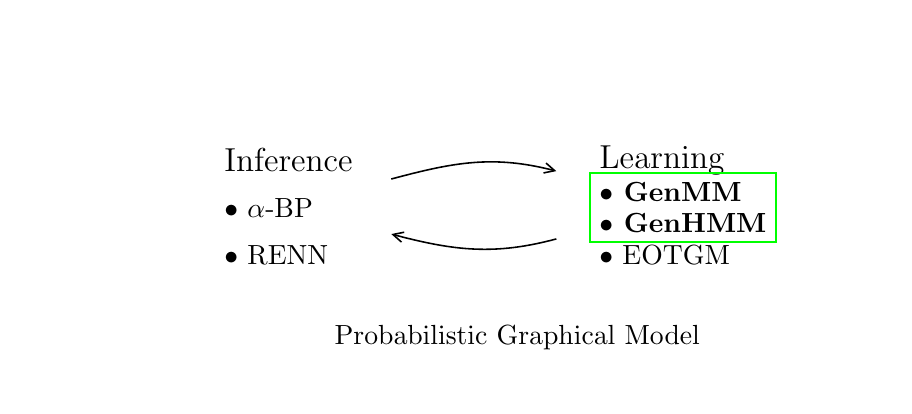
\begin{tikzpicture}
          \tikzstyle{cnode} = [thick, draw=white, ellipse, inner sep = 2pt,  align=center]
          \tikzstyle{fnode} = [thick, draw=white, ellipse, inner sep = 10pt,  align=center]
          \tikzstyle{rnode} = [thick, rectangle, inner sep = 1.5pt,  align=left]
          \node[rnode] (inf) at (-2, 0) {\large Inference};
          \node[rnode, below = 0.6cm of inf.west, anchor=west] (abp) {$\bullet$ {$\alpha$-BP}};
          \node[rnode, below = 1.2cm of inf.west, anchor=west] (renn) {$\bullet$ RENN};
          \node[cnode, fit=(abp)(inf)(renn)] (infn) {};
          
          \node[rnode, right = 3 of inf] (lern) {\large Learning};
          \node[rnode, below = 0.4 of lern.west, anchor=west] (genmm) {\textbf{$\bullet$ GenMM}};
          \node[rnode, below = 0.8 of lern.west, anchor=west] (genhmm) {\textbf{{$\bullet$} GenHMM}};
          \node[rnode, below = 1.2 of lern.west, anchor=west] (lfree) {{$\bullet$} EOTGM};
          \node[cnode, fit=(lern)(genmm)(genhmm)(lfree)] (learn) {};
          \node[rnode, draw=green, fit=(genmm)(genhmm)] () {};

          \node[fnode, fit=(infn)(lern)] (box) {};

          
          \node[below right = 0.5 and -0.5 of infn] {{Probabilistic} Graphical Model};
          \draw[->,line width=0.2mm] (infn) to[out=15, in=165] (learn);
          \draw[->,line width=0.2mm] (learn) to[out=195, in=-15] (infn);
        \end{tikzpicture}
      }
    \end{center}
    
  \end{frame}
}
\begin{frame}[label=current]
  {Incomplete Observation}
  Partial observation: $\bm{x} = [  \underbrace{\bm{x}_U}_{Unobserved}, \underbrace{\bm{x}_O}_{Observed}]$
  \begin{equation*}
    l(\bm{x}_O; \bm{\theta}) = \log{\sum_{\bm{x}_U}p(\bm{x}_U, \bm{x}_O; \bm{\theta})} = \log{\underbrace{Z(\bm{x}_O;\bm{\theta})}_{\sum_{\bm{x}_U}\tilde{p}(\bm{x}; \bm{\theta})}} - \log{Z(\bm{\theta})},
  \end{equation*}

  {Connect Free Energy to Evidence Lower Bounder}:
  \begin{columns}
    \column{0.6\textwidth}
    \begin{align*}
      l(\bm{x}_O; \bm{\theta}) &\geq - \underbrace{F_v(q(\bm{x}_U|\bm{x}_O))}_{Variational Free Energy} - \log{Z(\bm{\theta})} \nonumber \\
                               & = \EE_{q(\bm{x}_U|\bm{x}_O)}\left[ \log{\frac{{p}(\bm{x}_U, \bm{x}_O; \bm{\theta})}{q(\bm{x}_U|\bm{x}_O)}} \right] \nonumber \\
                               & = \underbrace{\EE_{q(\bm{x}_U|\bm{x}_O)}\left[ \log{{p}(\bm{x}_U, \bm{x}_O; \bm{\theta})} \right] + H({q(\bm{x}_U|\bm{x}_O)})}_{\text{Evidence Lower Bound $F(q, \bm{\theta})$}}
    \end{align*}
    
    \column{0.4\textwidth}
    Intuition of maximizing $F(q,\bm{\theta})$
    \begin{itemize}[label=\textbullet]
    \item Maximizing (incomplete) likelihood
    \item Minimizing free energy
    \end{itemize}

  \end{columns}
  This gives the EM as a coordinate ascent method:
  \begin{align*}
    \mathrm{E~step:}~~~ q^{(t+1)} &= \uargmax{q}{F(q, \bm{\theta}^{(t)})}, \\
    \mathrm{M~step:}~~~\bm{\theta}^{(t+1)} &= \uargmax{\bm{\theta}}{F(q^{(t+1)}, \bm{\theta})}.
  \end{align*}
\end{frame}


\begin{frame}[label=current]{Generator Mixed Model}
  {Equipping EM with Normalizing Flows}
  \begin{columns}
    \column{0.4\textwidth}
    \centering
    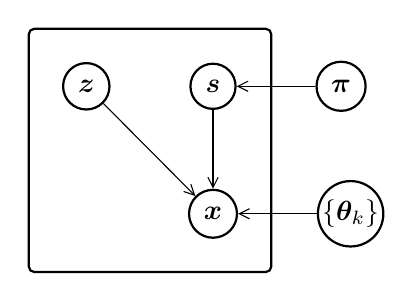
\begin{tikzpicture}
      \tikzstyle{enode} = [thick, draw=black, circle, align=center]
      \tikzstyle{cnode} = [thick, draw=black, circle, align=center, inner sep = 0.3pt]
      \tikzstyle{nnode} = [thick, rectangle, rounded corners = 2pt,minimum size = 0.8cm,draw,inner sep = 12pt]
      %%%%%%%%%%%%%%%%%%%%%%%%%%%%%%%%%%%%%%%% 
      %% directed graphical model
      %%%%%%%%%%%%%%%%%%%%%%%%%%%%%%%%%%%%%%%% 
      \begin{scope}[scale=1, every node/.append style={transform shape}]
        \node[enode] (x) at (0,0){$\bm{x}$};

\node[enode, above=of x] (s) {$\bm{s}$};
\node[enode, left=of s] (z) {$\bm{z}$};
\node[enode, right=of s] (pi) {$\bm{\pi}$};
\node[cnode, right=of x] (phi) {$\{ \bm{\theta}_k \}$};
\node[nnode, fit=(x)(z)(s)] (box) {};

\draw[->] (z) to (x);
\draw[->] (s) to (x);
\draw[->] (pi) to (s);
\draw[->] (phi) to (x);

%%% Local Variables:
%%% mode: latex
%%% TeX-master: "../ppgm_slide"
%%% End:

      \end{scope}

    \end{tikzpicture}
    
    \column{0.55\textwidth}
    
    \centering
    \begin{minipage}{\linewidth}
      
      \begin{itemize}[label=\textbullet]
      \item Ideal case: The underline true $p^{\ast}(\bm{x})$ is in hypothesis space $\Hh$, i.e. $p^{\ast}(\bm{x}) \in \Hh$.
      \item Out of reach: Test $p^{\ast}(\bm{x}) \stackrel{?}{\in} \Hh$
      \item A general desire:
        \begin{equation*}
          \Hh ~\mathrm{is~large}  \rightarrow \mathrm{condidate}~ p(\bm{x};\bm{\theta})~\mathrm{is~flexible}
        \end{equation*}
        
      \end{itemize}
      
      This brings up the finite \textbf{mixture} models.

      \begin{align*}\label{eq:FirstMixtureModel}
        p(\bm{x};\bm{\Theta})  = \textstyle\sum_{k=1}^K \pi_k  p_k(\bm{x}) = \textstyle \sum_{k=1}^K \pi_k  p(\underbrace{\bm{g}(\bm{z};\bm{\theta}_k)}_{\text{\begin{tabular}{c}Variable change \\via generator $\bm{g}$\end{tabular}}}).
      \end{align*}
      
    \end{minipage}
  \end{columns}
  
  \vskip -0.5cm
  What to expect from GenMM:
  \begin{itemize}[label=\textbullet]
  \item {Flexible and expressive model, enlarging hyperspace $\Hh$}
  \item {Tractable likelihood} 
  \item {Compatible with typical statistical models}
  \item Compatible with NN tools/frameworks
  \item {Scale to high-dimensional structured data}
  \item {Efficient in sampling (data generation)}
  \item {...}
  \end{itemize}

\end{frame}




\begin{frame}[label=current]{A High-level View of GenMM: finite mixture}
  \begin{tikzpicture}
    \tikzstyle{enode} = [thick, draw=black, circle, align=center]
    \tikzstyle{cnode} = [thick, draw=black, circle, align=center, inner sep = 0.3pt]
    \tikzstyle{nnode} = [thick, rectangle, rounded corners = 2pt,minimum size = 0.8cm,draw,inner sep = 22pt]
    %%%%%%%%%%%%%%%%%%%%%%%%%%%%%%%%%%%%%%%% 
    %% 1. directed graphical model
    %%%%%%%%%%%%%%%%%%%%%%%%%%%%%%%%%%%%%%%% 
    \begin{scope}[scale=0.6, every node/.append style={transform shape}, local bounding box=dgm, opacity=0.3]
      \node[enode] (x) at (0,0){$\bm{x}$};

\node[enode, above=of x] (s) {$\bm{s}$};
\node[enode, left=of s] (z) {$\bm{z}$};
\node[enode, right=of s] (pi) {$\bm{\pi}$};
\node[cnode, right=of x] (phi) {$\{ \bm{\theta}_k \}$};
\node[nnode, fit=(x)(z)(s)] (box) {};

\draw[->] (z) to (x);
\draw[->] (s) to (x);
\draw[->] (pi) to (s);
\draw[->] (phi) to (x);

%%% Local Variables:
%%% mode: latex
%%% TeX-master: "../ppgm_slide"
%%% End:

    \end{scope}
    
    %%%%%%%%%%%%%%%%%%%%%%%%%%%%%%%%%%%%%%%% 
    %% 2. illustration of GenMM
    %%%%%%%%%%%%%%%%%%%%%%%%%%%%%%%%%%%%%%%% 
    \begin{scope}[shift={($(dgm.east)+(3cm,0)$)}, local bounding box=illsGenMM]
      
% \tikzstyle{enode} = [thick, draw=blue, circle, inner sep = 3pt,
% align=center]
\tikzstyle{enode} = [thick, draw=black, ellipse, inner sep = 2pt,  align=center]
\tikzstyle{nnode} = [thick, rectangle, rounded corners = 2pt,minimum size = 0.8cm,draw,inner sep = 2pt]
\node[enode,label={below:{\tiny Shared latent source}}] (z) at (0,0) {$\bm{z}\sim p(\bm{z})$};
\node[enode, label={below:{\tiny Induced distribution}}] (x) at (5.5,0){$\bm{x}\sim p(\bm{x}; \bm{\Phi})$};
% \node at (5.2,-1) {$p(\bm{x};\bm{\Phi}) = \textstyle\sum_{k=1}^K \pi_k  p_k(\bm{x})$};
\node[nnode] (g1) at (2.6,1.8) {$\bm{g}_1$};
\node[nnode] (g2) at (2.6,0.5) {$\bm{g}_2$};
\node[nnode] (gk) at (2.6,-1.8) {$\bm{g}_K$};
\draw[dotted,line width=2pt] (2.6,-0.3) -- (2.6,-1.2);
\draw[->] (z) [in= 180, out =0] to (g1);
\draw[->] (z) [in= 180, out =0] to (g2);
\draw[->] (z) [in= 180, out =0] to (gk);
\filldraw[->] (3.7, 0.5)circle (2pt) -- node[above=0.2](switch){$\bm{s}\sim \bm{\pi}$} (x);
\node[above= 0.2 of switch.east] {\tiny \begin{tabular}{c}Categorical variable\\ as generator switch\end{tabular}};
% \draw[->] (3,-0.8) -- (3.5, -0.8);
\draw[->] (g1) -- (3.5,1.8);
\draw[->] (g2) -- (3.5, 0.5);
\draw[->] (gk) -- (3.5, -1.8);
\begin{scope}[on background layer, every node/.append style={transform shape}]
\node [rounded corners = 2pt, inner sep=4pt, fill=blue!30,fit=(g1)(g2)(gk), label={[label distance=0.3cm]-60:{\tiny Mixture of generators}}] {};
\end{scope}
%%% Local Variables:
%%% mode: latex
%%% TeX-master: "../ppgm_slide"
%%% End:

    \end{scope}
    \draw[green, ->, shorten >=5pt, shorten <=5pt] (dgm) --node [text width=2cm, black, midway,above]{\tiny Alternative illustration of GenMM} (illsGenMM);
    
    %%%%%%%%%%%%%%%%%%%%%%%%%%%%%%%%%%%%%%%% 
    %% 3. illustration of flow
    %%%%%%%%%%%%%%%%%%%%%%%%%%%%%%%%%%%%%%%% 

    \begin{scope}[shift={($(illsGenMM.south)+(-1cm,-1cm)$)}, scale=0.8, local bounding box=illFlow,opacity=\bgopacity]
      \def\layersep{1.5cm}
\begin{scope}[shorten >=1pt,->,draw=black!50, node distance=\layersep, scale=0.6, every node/.append style={transform shape},transform shape, local bounding box=ffnn]
  \tikzstyle{every pin edge}=[<-,shorten <=1pt]
  \tikzstyle{neuron}=[circle,fill=black!50,minimum size=17pt,inner sep=0pt]
  \tikzstyle{input neuron}=[neuron, fill=green!80];
  \tikzstyle{output neuron}=[neuron, fill=red!80];
  \tikzstyle{hidden neuron}=[neuron, fill=blue!80];
  \tikzstyle{annot} = [text width=4em, text centered]

  % Draw the input layer nodes
  \foreach \name / \y in {1,...,4}
  % This is the same as writing \foreach \name / \y in {1/1,2/2,3/3,4/4}
  % \node[input neuron, pin=left:Input \#\y] (I-\name) at (0,-\y) {};
  \node[input neuron, pin=left:{}] (I-\name) at (0,-\y) {};


  % Draw the hidden layer nodes
  \foreach \name / \y in {1,...,4}
  \path[yshift=0.0cm] node[hidden neuron] (H-\name) at (\layersep,-\y cm) {};

  % Draw the output layer node
  \foreach \name / \y in {1,...,4}
  \node[output neuron,pin={[pin edge={->}]right:{}}] (O-\name) at (2*\layersep, -\y cm) {};

  % Connect every node in the input layer with every node in the
  % hidden layer.
  \foreach \source in {1,...,4}
  \foreach \dest in {1,...,4}
  \draw[-{Stealth[scale=0.5]}] (I-\source) edge (H-\dest);

  % Connect every node in the hidden layer with the output layer
  \foreach \source in {1,...,4}
  \foreach \dest in {1,...,4}
  \draw[-{Stealth[scale=0.5]}] (H-\source) edge (O-\dest);

  % \foreach \source in {1,...,4}
  % \path (H-\source) edge (O);

  % Annotate the layers
  % \node[annot,above of=H-1, node distance=1cm] (hl) {Hidden layer};
  % \node[annot,left of=hl] {Input layer};
  % \node[annot,right of=hl] {Output layer};
  
\end{scope}
\node[inner sep=0pt, left= 0.2cm of ffnn] (latentz) {\includegraphics[width=.2\textwidth]{images/moon/zdist-crop.pdf}};
\node[inner sep=0pt, right= 0.2cm of ffnn] (latentx) {\includegraphics[width=.2\textwidth]{images/moon/xdist-crop.pdf}};
%%% Local Variables:
%%% mode: latex
%%% TeX-master: "../ppgm_slide"
%%% End:

    \end{scope}
    
    \draw[dashed, ->, shorten >=5pt, shorten <=5pt, opacity=\bgopacity] ($(gk.north)+(0,-1.0cm)$) -- ($(gk.north)+(0,-2.0cm)$);
    
    %%%%%%%%%%%%%%%%%%%%%%%%%%%%%%%%%%%%%%%% 
    %% 4. one layer mapping of the flow
    %%%%%%%%%%%%%%%%%%%%%%%%%%%%%%%%%%%%%%%% 
    \draw[dashed, ->, shorten >=5pt, shorten <=5pt, opacity=\bgopacity] ($(latentz.west)+(-0.1cm,0)$) -- ($(latentz.west)+(-1.5cm,0)$);
    
    \begin{scope}[shift={($(dgm.south)+(0,-3.5cm)$)}, scale=0.5, every node/.append style={transform shape}, local bounding box=oneLayer, opacity=\bgopacity]
      \input{sections/genmm4.tex}
    \end{scope}
    
  \end{tikzpicture}
\end{frame}


\begin{frame}[label=current]{A High-level View of GenMM: flow gears}
  \begin{tikzpicture}
    \tikzstyle{enode} = [thick, draw=black, circle, align=center]
    \tikzstyle{cnode} = [thick, draw=black, circle, align=center, inner sep = 0.3pt]
    \tikzstyle{nnode} = [thick, rectangle, rounded corners = 2pt,minimum size = 0.8cm,draw,inner sep = 22pt]
    %%%%%%%%%%%%%%%%%%%%%%%%%%%%%%%%%%%%%%%% 
    %% 1. directed graphical model
    %%%%%%%%%%%%%%%%%%%%%%%%%%%%%%%%%%%%%%%% 
    \begin{scope}[scale=0.4, every node/.append style={transform shape}, local bounding box=dgm, opacity=0.3]
      \node[enode] (x) at (0,0){$\bm{x}$};

\node[enode, above=of x] (s) {$\bm{s}$};
\node[enode, left=of s] (z) {$\bm{z}$};
\node[enode, right=of s] (pi) {$\bm{\pi}$};
\node[cnode, right=of x] (phi) {$\{ \bm{\theta}_k \}$};
\node[nnode, fit=(x)(z)(s)] (box) {};

\draw[->] (z) to (x);
\draw[->] (s) to (x);
\draw[->] (pi) to (s);
\draw[->] (phi) to (x);

%%% Local Variables:
%%% mode: latex
%%% TeX-master: "../ppgm_slide"
%%% End:

    \end{scope}
    
    %%%%%%%%%%%%%%%%%%%%%%%%%%%%%%%%%%%%%%%% 
    %% 2. illustration of GenMM
    %%%%%%%%%%%%%%%%%%%%%%%%%%%%%%%%%%%%%%%% 
    \begin{scope}[scale=0.3, every node/.append style={transform shape}, shift={($(dgm.east)+(16cm,0)$)}, local bounding box=illsGenMM, opacity=\bgopacity]
      
% \tikzstyle{enode} = [thick, draw=blue, circle, inner sep = 3pt,
% align=center]
\tikzstyle{enode} = [thick, draw=black, ellipse, inner sep = 2pt,  align=center]
\tikzstyle{nnode} = [thick, rectangle, rounded corners = 2pt,minimum size = 0.8cm,draw,inner sep = 2pt]
\node[enode,label={below:{\tiny Shared latent source}}] (z) at (0,0) {$\bm{z}\sim p(\bm{z})$};
\node[enode, label={below:{\tiny Induced distribution}}] (x) at (5.5,0){$\bm{x}\sim p(\bm{x}; \bm{\Phi})$};
% \node at (5.2,-1) {$p(\bm{x};\bm{\Phi}) = \textstyle\sum_{k=1}^K \pi_k  p_k(\bm{x})$};
\node[nnode] (g1) at (2.6,1.8) {$\bm{g}_1$};
\node[nnode] (g2) at (2.6,0.5) {$\bm{g}_2$};
\node[nnode] (gk) at (2.6,-1.8) {$\bm{g}_K$};
\draw[dotted,line width=2pt] (2.6,-0.3) -- (2.6,-1.2);
\draw[->] (z) [in= 180, out =0] to (g1);
\draw[->] (z) [in= 180, out =0] to (g2);
\draw[->] (z) [in= 180, out =0] to (gk);
\filldraw[->] (3.7, 0.5)circle (2pt) -- node[above=0.2](switch){$\bm{s}\sim \bm{\pi}$} (x);
\node[above= 0.2 of switch.east] {\tiny \begin{tabular}{c}Categorical variable\\ as generator switch\end{tabular}};
% \draw[->] (3,-0.8) -- (3.5, -0.8);
\draw[->] (g1) -- (3.5,1.8);
\draw[->] (g2) -- (3.5, 0.5);
\draw[->] (gk) -- (3.5, -1.8);
\begin{scope}[on background layer, every node/.append style={transform shape}]
\node [rounded corners = 2pt, inner sep=4pt, fill=blue!30,fit=(g1)(g2)(gk), label={[label distance=0.3cm]-60:{\tiny Mixture of generators}}] {};
\end{scope}
%%% Local Variables:
%%% mode: latex
%%% TeX-master: "../ppgm_slide"
%%% End:

    \end{scope}
    \draw[dashed, ->, shorten >=5pt, shorten <=5pt, opacity=\bgopacity] (dgm) --node [text width=2cm, black, midway,above]{} (illsGenMM);
    
    %%%%%%%%%%%%%%%%%%%%%%%%%%%%%%%%%%%%%%%% 
    %% 3. illustration of flow
    %%%%%%%%%%%%%%%%%%%%%%%%%%%%%%%%%%%%%%%% 

    \begin{scope}[shift={($(illsGenMM.south)+(-0.5cm,0cm)$)}, scale=0.8, local bounding box=illFlow]
      \def\layersep{1.5cm}
\begin{scope}[shorten >=1pt,->,draw=black!50, node distance=\layersep, scale=0.6, every node/.append style={transform shape},transform shape, local bounding box=ffnn]
  \tikzstyle{every pin edge}=[<-,shorten <=1pt]
  \tikzstyle{neuron}=[circle,fill=black!50,minimum size=17pt,inner sep=0pt]
  \tikzstyle{input neuron}=[neuron, fill=green!80];
  \tikzstyle{output neuron}=[neuron, fill=red!80];
  \tikzstyle{hidden neuron}=[neuron, fill=blue!80];
  \tikzstyle{annot} = [text width=4em, text centered]

  % Draw the input layer nodes
  \foreach \name / \y in {1,...,4}
  % This is the same as writing \foreach \name / \y in {1/1,2/2,3/3,4/4}
  % \node[input neuron, pin=left:Input \#\y] (I-\name) at (0,-\y) {};
  \node[input neuron, pin=left:{}] (I-\name) at (0,-\y) {};


  % Draw the hidden layer nodes
  \foreach \name / \y in {1,...,4}
  \path[yshift=0.0cm] node[hidden neuron] (H-\name) at (\layersep,-\y cm) {};

  % Draw the output layer node
  \foreach \name / \y in {1,...,4}
  \node[output neuron,pin={[pin edge={->}]right:{}}] (O-\name) at (2*\layersep, -\y cm) {};

  % Connect every node in the input layer with every node in the
  % hidden layer.
  \foreach \source in {1,...,4}
  \foreach \dest in {1,...,4}
  \draw[-{Stealth[scale=0.5]}] (I-\source) edge (H-\dest);

  % Connect every node in the hidden layer with the output layer
  \foreach \source in {1,...,4}
  \foreach \dest in {1,...,4}
  \draw[-{Stealth[scale=0.5]}] (H-\source) edge (O-\dest);

  % \foreach \source in {1,...,4}
  % \path (H-\source) edge (O);

  % Annotate the layers
  % \node[annot,above of=H-1, node distance=1cm] (hl) {Hidden layer};
  % \node[annot,left of=hl] {Input layer};
  % \node[annot,right of=hl] {Output layer};
  
\end{scope}
\node[inner sep=0pt, left= 0.2cm of ffnn] (latentz) {\includegraphics[width=.2\textwidth]{images/moon/zdist-crop.pdf}};
\node[inner sep=0pt, right= 0.2cm of ffnn] (latentx) {\includegraphics[width=.2\textwidth]{images/moon/xdist-crop.pdf}};
%%% Local Variables:
%%% mode: latex
%%% TeX-master: "../ppgm_slide"
%%% End:

    \end{scope}
    \node [black, below=-0.05cm of illFlow] (changeveq) {
      \scriptsize
      \begin{minipage}{0.7\textwidth}
        When the $k$-th generator is selected, i.e., $s_k=1$ and $s_{k^{\prime}}=0$  for $k^{\prime}\neq k$, say $\tilde{\bm{x}} = \bm{x}|_{s_k=1}$. By following the \href{https://online.stat.psu.edu/stat414/lesson/23/23.1}{change of variable rule}
        \vskip -0.4cm
        \begin{equation*}
          \underbrace{p(\tilde{\bm{x}})|_{\tilde{\bm{x}} = \tilde{\bm{g}}(\bm{z})}}_{\text{Induced distribution}} =  \underbrace{p(\bm{z})}_{\text{\begin{tabular}{c}Assumed known distribution \\ easy to sample\end{tabular}}}\cdot \underbrace{\bigg| \mathrm{det}\left({\pd{\bm{z}}{\tilde{\bm{x}}}}\right)\bigg|}_{\text{\begin{tabular}{c}Computational load\\ depends on the mapping\end{tabular}}}.
        \end{equation*}
        \only<1>{
          \vskip -0.4cm
          A toy example:\\
        }
        \only<2>{
          \vskip -0.4cm
          Powering it with a $L$-layer neural network implementation:
        }
      \end{minipage}};
    \draw[green, ->, shorten >=5pt, shorten <=5pt] ($(gk.north)+(0,0cm)$) -- ($(gk.north)+(0,-0.8cm)$);
    \only<1>{
      \begin{scope}[scale=0.8, shift={($(changeveq.south)+(-2.5cm,-0.7cm)$)}]
        \node[black] at (2.5cm, 0) {\scriptsize
          Gaussian linear transform: $Z \sim \mathsf{N}\left( 0, 1  \right)$ $\xrightarrow{X=\sigma\cdot Z + \mu}$ $X \sim \mathsf{N}\left( \mu, \sigma  \right)$
        };
      \end{scope}
    }
    \only<2>{
      \begin{scope}[scale=0.8, shift={($(changeveq.south)+(-2.5cm,-0.7cm)$)}]
        \node (z) at (0,0) {};
        \node at ($(z)-(0.5,0)$){$\bm{z}=\bm{h}_0$};
        \node (xi1) at (1.5,0) {$\bm{h}_1$};
        \node (xi2) at (3,0) {};
        \node (xi3) at (4.5,0){};
        \node (x) at (6,0) {};
        \node at ($(x)+(0.5,0)$){$\bm{x} = \bm{h}_L$};
        \draw[->] ($(z) + (0.3,0.1)$) -- node[above]{$\tilde{\bm{g}}_1$} ($(xi1)+(-0.3,0.1)$); 
        \draw[->] ($(xi1)-(0.3,0.1)$) -- node[below]{$\tilde{\bm{f}}_1$}($(z) - (-0.3,0.1)$);
        \draw[->] ($(xi1) + (0.3,0.1)$) -- node[above]{$\tilde{\bm{g}}_2$} ($(xi2)+(-0.3,0.1)$); 
        \draw[->] ($(xi2)-(0.3,0.1)$) -- node[below]{$\tilde{\bm{f}}_2$}($(xi1) - (-0.3,0.1)$);
        \draw[->] ($(xi3) + (0.3,0.1)$) -- node[above]{$\tilde{\bm{g}}_L$} ($(x)+(-0.3,0.1)$); 
        \draw[->] ($(x)-(0.3,0.1)$) -- node[below]{$\tilde{\bm{f}}_L$}($(xi3) - (-0.3,0.1)$);
        \draw[dotted,line width = 0.3 mm] (xi2) -- (xi3);
      \end{scope}
    }
    %%%%%%%%%%%%%%%%%%%%%%%%%%%%%%%%%%%%%%%% 
    %% 4. one layer mapping of the flow
    %%%%%%%%%%%%%%%%%%%%%%%%%%%%%%%%%%%%%%%% 
    
    \begin{scope}[shift={($(dgm.south)+(0,-3.5cm)$)}, scale=0.3, every node/.append style={transform shape}, local bounding box=oneLayer, opacity=\bgopacity]
      \input{sections/genmm4.tex}
    \end{scope}
    \draw[dashed, ->, shorten >=5pt, shorten <=5pt, opacity=\bgopacity] ($(oneLayer.east)+(1.5cm,0cm)$) -- ($(oneLayer.east)+(0.1cm,0)$);
    
  \end{tikzpicture}
\end{frame}



\begin{frame}[label=current]{A High-level View of GenMM: Zoom into Layer}
  \begin{tikzpicture}
    \tikzstyle{enode} = [thick, draw=black, circle, align=center]
    \tikzstyle{cnode} = [thick, draw=black, circle, align=center, inner sep = 0.3pt]
    \tikzstyle{nnode} = [thick, rectangle, rounded corners = 2pt,minimum size = 0.8cm,draw,inner sep = 22pt]
    %%%%%%%%%%%%%%%%%%%%%%%%%%%%%%%%%%%%%%%% 
    %% 1. directed graphical model
    %%%%%%%%%%%%%%%%%%%%%%%%%%%%%%%%%%%%%%%% 
    \begin{scope}[scale=0.4, every node/.append style={transform shape}, local bounding box=dgm, opacity=0.3]
      \node[enode] (x) at (0,0){$\bm{x}$};

\node[enode, above=of x] (s) {$\bm{s}$};
\node[enode, left=of s] (z) {$\bm{z}$};
\node[enode, right=of s] (pi) {$\bm{\pi}$};
\node[cnode, right=of x] (phi) {$\{ \bm{\theta}_k \}$};
\node[nnode, fit=(x)(z)(s)] (box) {};

\draw[->] (z) to (x);
\draw[->] (s) to (x);
\draw[->] (pi) to (s);
\draw[->] (phi) to (x);

%%% Local Variables:
%%% mode: latex
%%% TeX-master: "../ppgm_slide"
%%% End:

    \end{scope}
    
    %%%%%%%%%%%%%%%%%%%%%%%%%%%%%%%%%%%%%%%% 
    %% 2. illustration of GenMM
    %%%%%%%%%%%%%%%%%%%%%%%%%%%%%%%%%%%%%%%% 
    \begin{scope}[scale=0.3, every node/.append style={transform shape}, shift={($(dgm.east)+(20cm,0)$)}, local bounding box=illsGenMM, opacity=\bgopacity]
      
% \tikzstyle{enode} = [thick, draw=blue, circle, inner sep = 3pt,
% align=center]
\tikzstyle{enode} = [thick, draw=black, ellipse, inner sep = 2pt,  align=center]
\tikzstyle{nnode} = [thick, rectangle, rounded corners = 2pt,minimum size = 0.8cm,draw,inner sep = 2pt]
\node[enode,label={below:{\tiny Shared latent source}}] (z) at (0,0) {$\bm{z}\sim p(\bm{z})$};
\node[enode, label={below:{\tiny Induced distribution}}] (x) at (5.5,0){$\bm{x}\sim p(\bm{x}; \bm{\Phi})$};
% \node at (5.2,-1) {$p(\bm{x};\bm{\Phi}) = \textstyle\sum_{k=1}^K \pi_k  p_k(\bm{x})$};
\node[nnode] (g1) at (2.6,1.8) {$\bm{g}_1$};
\node[nnode] (g2) at (2.6,0.5) {$\bm{g}_2$};
\node[nnode] (gk) at (2.6,-1.8) {$\bm{g}_K$};
\draw[dotted,line width=2pt] (2.6,-0.3) -- (2.6,-1.2);
\draw[->] (z) [in= 180, out =0] to (g1);
\draw[->] (z) [in= 180, out =0] to (g2);
\draw[->] (z) [in= 180, out =0] to (gk);
\filldraw[->] (3.7, 0.5)circle (2pt) -- node[above=0.2](switch){$\bm{s}\sim \bm{\pi}$} (x);
\node[above= 0.2 of switch.east] {\tiny \begin{tabular}{c}Categorical variable\\ as generator switch\end{tabular}};
% \draw[->] (3,-0.8) -- (3.5, -0.8);
\draw[->] (g1) -- (3.5,1.8);
\draw[->] (g2) -- (3.5, 0.5);
\draw[->] (gk) -- (3.5, -1.8);
\begin{scope}[on background layer, every node/.append style={transform shape}]
\node [rounded corners = 2pt, inner sep=4pt, fill=blue!30,fit=(g1)(g2)(gk), label={[label distance=0.3cm]-60:{\tiny Mixture of generators}}] {};
\end{scope}
%%% Local Variables:
%%% mode: latex
%%% TeX-master: "../ppgm_slide"
%%% End:

    \end{scope}
    \draw[dashed, ->, shorten >=5pt, shorten <=5pt, opacity=\bgopacity] (dgm) --node [text width=2cm, black, midway,above]{} (illsGenMM);
    
    %%%%%%%%%%%%%%%%%%%%%%%%%%%%%%%%%%%%%%%% 
    %% 3. illustration of flow
    %%%%%%%%%%%%%%%%%%%%%%%%%%%%%%%%%%%%%%%% 

    \begin{scope}[shift={($(illsGenMM.south)+(-0.5cm,0cm)$)}, scale=0.5, local bounding box=illFlow, opacity=\bgopacity]
      \def\layersep{1.5cm}
\begin{scope}[shorten >=1pt,->,draw=black!50, node distance=\layersep, scale=0.6, every node/.append style={transform shape},transform shape, local bounding box=ffnn]
  \tikzstyle{every pin edge}=[<-,shorten <=1pt]
  \tikzstyle{neuron}=[circle,fill=black!50,minimum size=17pt,inner sep=0pt]
  \tikzstyle{input neuron}=[neuron, fill=green!80];
  \tikzstyle{output neuron}=[neuron, fill=red!80];
  \tikzstyle{hidden neuron}=[neuron, fill=blue!80];
  \tikzstyle{annot} = [text width=4em, text centered]

  % Draw the input layer nodes
  \foreach \name / \y in {1,...,4}
  % This is the same as writing \foreach \name / \y in {1/1,2/2,3/3,4/4}
  % \node[input neuron, pin=left:Input \#\y] (I-\name) at (0,-\y) {};
  \node[input neuron, pin=left:{}] (I-\name) at (0,-\y) {};


  % Draw the hidden layer nodes
  \foreach \name / \y in {1,...,4}
  \path[yshift=0.0cm] node[hidden neuron] (H-\name) at (\layersep,-\y cm) {};

  % Draw the output layer node
  \foreach \name / \y in {1,...,4}
  \node[output neuron,pin={[pin edge={->}]right:{}}] (O-\name) at (2*\layersep, -\y cm) {};

  % Connect every node in the input layer with every node in the
  % hidden layer.
  \foreach \source in {1,...,4}
  \foreach \dest in {1,...,4}
  \draw[-{Stealth[scale=0.5]}] (I-\source) edge (H-\dest);

  % Connect every node in the hidden layer with the output layer
  \foreach \source in {1,...,4}
  \foreach \dest in {1,...,4}
  \draw[-{Stealth[scale=0.5]}] (H-\source) edge (O-\dest);

  % \foreach \source in {1,...,4}
  % \path (H-\source) edge (O);

  % Annotate the layers
  % \node[annot,above of=H-1, node distance=1cm] (hl) {Hidden layer};
  % \node[annot,left of=hl] {Input layer};
  % \node[annot,right of=hl] {Output layer};
  
\end{scope}
\node[inner sep=0pt, left= 0.2cm of ffnn] (latentz) {\includegraphics[width=.2\textwidth]{images/moon/zdist-crop.pdf}};
\node[inner sep=0pt, right= 0.2cm of ffnn] (latentx) {\includegraphics[width=.2\textwidth]{images/moon/xdist-crop.pdf}};
%%% Local Variables:
%%% mode: latex
%%% TeX-master: "../ppgm_slide"
%%% End:

    \end{scope}
    \draw[dashed, ->, shorten >=5pt, shorten <=5pt, opacity=\bgopacity] ($(gk.north)+(0,0cm)$) -- ($(gk.north)+(0,-0.8cm)$);
    %%%%%%%%%%%%%%%%%%%%%%%%%%%%%%%%%%%%%%%% 
    %% 4. one layer mapping of the flow
    %%%%%%%%%%%%%%%%%%%%%%%%%%%%%%%%%%%%%%%% 
    
    \begin{scope}[shift={($(dgm.south)+(0,-1.5cm)$)}, scale=0.7, every node/.append style={transform shape}, local bounding box=oneLayer]
      \input{sections/genmm4.tex}
    \end{scope}
    \node [black, right=-0.5cm of oneLayer.east] {\scriptsize{Forward}};
    \node [black, below=1.3cm of oneLayer.west,anchor=west] (forwardmap) {
      \tiny
      \begin{minipage}{0.4\linewidth}
        \begin{equation*}
          \bm{h}_{l-1} =
          \begin{bmatrix}
            \bm{h}_{l-1,a}\\
            \bm{h}_{l-1,b}
          \end{bmatrix}
          =
          \begin{bmatrix}
            \bm{h}_{l,a}\\
            \bm{m}_a(\bm{h}_{l,a})\odot \bm{h}_{l,b} + \bm{m}_b(\bm{h}_{l,a})
          \end{bmatrix}
        \end{equation*}
      \end{minipage}
    };
    
    \begin{scope}[shift={($(oneLayer.south)+(0,-2.0cm)$)}, scale=0.7, every node/.append style={transform shape}, local bounding box=oneLayerInverse]
      % \tikzstyle{enode} = [thick, draw=blue, circle, inner sep = 3pt,
% align=center]
\tikzstyle{enode} = [thick, draw, circle, inner sep = 0, minimum size = 1cm,  align=center]
\tikzstyle{nnode} = [thick, rectangle, rounded corners = 2pt,minimum size = 0.4cm,draw,inner sep = 2pt]
\node[enode] (hal) at (-2,1) {$\bm{h}_{l,a}$};
\node[enode] (hbl) at (-2,-1) {$\bm{h}_{l,b}$};
\node[enode] (hal-1) at (2,1) {$\bm{h}_{l-1,a}$};
\node[enode] (hbl-1) at (2,-1) {$\bm{h}_{l-1,b}$};
\node[nnode] (times) at (-0.5,-1) {$\div$};
\node[nnode] (plus) at (0.5,-1) {$-$};
\node[nnode] (eq) at (0,1) {$=$};
\draw[->] (hal-1) -- node[fill=white] {$\bm{m}_a$} (times);
\draw[->] (hal-1) -- node[fill=white] {$\bm{m}_b$} (plus);
\draw[<-] (hal) to (eq);

\draw[<-] (eq) to (hal-1);
\draw[->] (hbl) to (times);
\draw[<-] (times) to (plus);
\draw[<-] (plus) to (hbl-1);
% \draw[draw=black] (-0.5,-0.5) rectangle ++(1,2);


%%% Local Variables:
%%% mode: latex
%%% TeX-master: "../ppgm_slide"
%%% End:

    \end{scope}
    \node [black, right=-0.5cm of oneLayerInverse.east] {\scriptsize{Inverse}};

    \node [black, below=1.3cm of oneLayerInverse.west,anchor=west] (backwardmap) {
      \tiny
      \begin{minipage}{0.4\linewidth}
        \begin{equation*}
          \bm{h}_{l} =
          \begin{bmatrix}
            \bm{h}_{l,a}\\
            \bm{h}_{l,b}
          \end{bmatrix}
          =
          \begin{bmatrix}
            \bm{h}_{l-1,a}\\
            \left(  \bm{h}_{l-1,b} - \bm{m}_b(\bm{h}_{l-1,a}) \right)\oslash \bm{m}_a(\bm{h}_{l-1,a}) 
          \end{bmatrix}
        \end{equation*}
      \end{minipage}
    };

    \node [black, right=-0.5cm of oneLayerInverse.east] {\scriptsize{Inverse}};

    \node [black, right=2.3cm of oneLayerInverse.east,anchor=west] (attrtext) {
      \scriptsize
      \begin{minipage}{0.5\linewidth}
        \begin{itemize}[label=\textbullet]
        \item $\odot$ denotes element-wise product, $\oslash$ denotes
          element-wise division
        \item Mapping $\bm{m}_a$, $\bm{m}_b$ can be as complex as possible and not necessary invertible
        \item Same computation complexity of forward and inverse mapping
        \item Triangular matix of Jacobian
        \end{itemize}
        Alternative arch. on market: Auto-regressive flow, Glow, ODE, etc.
      \end{minipage}
    };
    \draw[green, ->] ($(oneLayer.east)+(3.5cm,0cm)$) --node [text width=5cm, black, right,above, anchor=north west]{\tiny Pick up one layer to zoom in} ($(oneLayer.east)+(1.1cm,0)$);
    
  \end{tikzpicture}
\end{frame}

\begin{frame}[label=current]
  {Alternative Mixture and Remark}
  \centering
  \begin{tikzpicture}[scale=0.7, every node/.append style={transform shape}]
    \tikzstyle{enode} = [thick, draw=black, ellipse, inner sep = 1pt,  align=center]
    \tikzstyle{nnode} = [thick, rectangle, rounded corners = 2pt,minimum size = 0.8cm,draw,inner sep = 2pt]
    \node[enode] (z1) at (0,1.8) {$\bm{z}\sim p_1(\bm{z})$};
    \node[enode] (z2) at (0,0.5){$\bm{z}\sim p_{2}(\bm{z})$};
    \node[enode] (zK) at (0,-1.8) {$\bm{z}\sim p_{K}(\bm{z})$}; 
    \node[enode, label={[label distance=0.3cm]-90:Induced Distribution}] (x) at (5.5,0){$\bm{x}\sim p(\bm{x};\ubar{\bm{\Phi}})$};
    
    \node[nnode, label={[label distance=0.5cm]-90:Share Generator}] (g) at (3.2,0) {$\bm{g}$};
    \draw[dotted,line width=2pt] (0,-0.3) -- (0,-1.2);
    \filldraw[->] (1.8, 0.5)circle (2pt) -- node[above=0.2]{$\bm{s}\sim \bm{\pi}$} (g) ;
    \draw[->] (z1) -- (1.6, 1.8);
    \draw[->] (z2) -- (1.6, 0.5);
    \draw[->] (zK) -- (1.6, -1.8);
    \begin{scope}[on background layer]
      \node[rounded corners = 4pt, rectangle, inner sep = 20pt,  align=center, fit=(z1)(z2)(zK), label=below:{Multiple Latent Sources}, fill=blue!30] (latSource) {};
    \end{scope}
    \draw[->] (g) to (x);
  \end{tikzpicture}
  
  \begin{block}{Remark On GenMM/GenHMM}
    \begin{itemize}[label=\textbullet]
    \item Free dimension for flexibility: number of mixture + complexity of functional form of neural networks
    \item Compatible with statistic methods and neural network techniques (error back-propagation, optimizer)
    \item Embed batch-gradient descent into M-step
    \item Lack of closed-form update rule and generator changes at each gradient step. We tackle by maintaining old and new generators in EM steps
    \end{itemize}
    
  \end{block}
\end{frame}

\begin{frame}[label=current]{Remark}
  \begin{block}{A diagram of connections}
    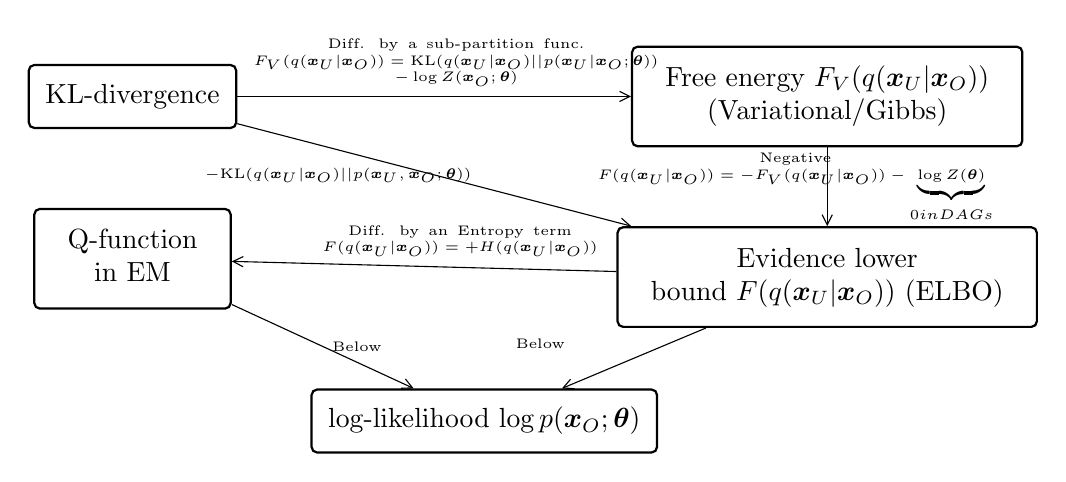
\begin{tikzpicture}
      \tikzstyle{cnode} = [thick, draw=black, circle, align=center, inner sep = 0.3pt]
      \tikzstyle{nnode} = [thick, rectangle, rounded corners = 2pt,minimum size = 0.8cm,draw,inner sep = 6pt]
      \node[nnode] (kl) at (0,0) {KL-divergence};
      \node[nnode, right= 5cm of kl] (freeEnergy) {\begin{tabular}{c}Free energy $F_V(q(\bm{x}_U|\bm{x}_O))$ \\ (Variational/Gibbs)\end{tabular}};
      \node[nnode, below= of freeEnergy] (elbo) {\begin{tabular}{c}Evidence lower\\ bound $F(q(\bm{x}_U|\bm{x}_O))$ (ELBO)\end{tabular}};
      \node[nnode, below= of kl] (q-fun) {\begin{tabular}{c}Q-function\\ in EM\end{tabular}};
      \node[nnode, below right= of q-fun] (llk) {log-likelihood $\log{p(\bm{x}_O;\bm{\theta})}$};
      \draw[black, ->] (kl) --node [text width=5cm, black, midway, above]{\tiny
        \begin{tabular}{c}
          Diff. by a sub-partition func. \\
          $F_V(q(\bm{x}_U|\bm{x}_O)) = \mathrm{KL}(q(\bm{x}_U|\bm{x}_O) || p(\bm{x}_U|\bm{x}_O; \bm{\theta})) $ \\
          $- \log{Z(\bm{x}_O; \bm{\theta})}$
        \end{tabular}}
      (freeEnergy);
      \draw[black, ->] (freeEnergy) --node [text width=3cm, black, midway, left]{\tiny
        \begin{tabular}{c}
          Negative \\
          $F(q(\bm{x}_U|\bm{x}_O)) = -F_V(q(\bm{x}_U|\bm{x}_O))- \underbrace{\log{Z(\bm{\theta})}}_{\text{0 in DAGs}}$
        \end{tabular}}
      (elbo);

      \draw[black, ->] (kl) --node [text width=3cm, black, midway, left]{\tiny
        \begin{tabular}{c}
          $-\mathrm{KL}(q(\bm{x}_U|\bm{x}_O) || p(\bm{x}_U,\bm{x}_O; \bm{\theta})) $
        \end{tabular}}
      (elbo);

      \draw[black, ->] (elbo) --node [text width=3cm, black, midway, above]{\tiny
        \begin{tabular}{c}
          Diff. by an Entropy term\\
          $F(q(\bm{x}_U|\bm{x}_O))= \Qq + H({q(\bm{x}_U|\bm{x}_O)})$
        \end{tabular}}
      (q-fun);

      \draw[black, ->] (elbo) --node [text width=3cm, black, midway, above]{\tiny
        Below
      }
      (llk);
      \draw[black, ->] (q-fun) --node [text width=3cm, black, midway, right]{\tiny
        Below
      }
      (llk);

      
    \end{tikzpicture}
    
  \end{block}
  \let\thefootnote\relax\footnotetext{\tiny
    \vskip -0.2cm
    A bit notation abuse, $\bm{x}_U$ corresponds to unobserved variable $\bm{z}$.
  }
\end{frame}


%%% Local Variables:
%%% mode: latex
%%% TeX-master: "../ppgm_slide"
%%% End:

\subsection{EOT}
{ \setbeamercolor{background canvas}{bg=hl_bg}
  \setbeamercolor{normal text}{fg=hl_fg}
  \setbeamercolor{frametitle}{fg=hl_fg}
  \begin{frame}[label=current]
    \usebeamercolor[fg]{normal text}
    \begin{center}
      {
        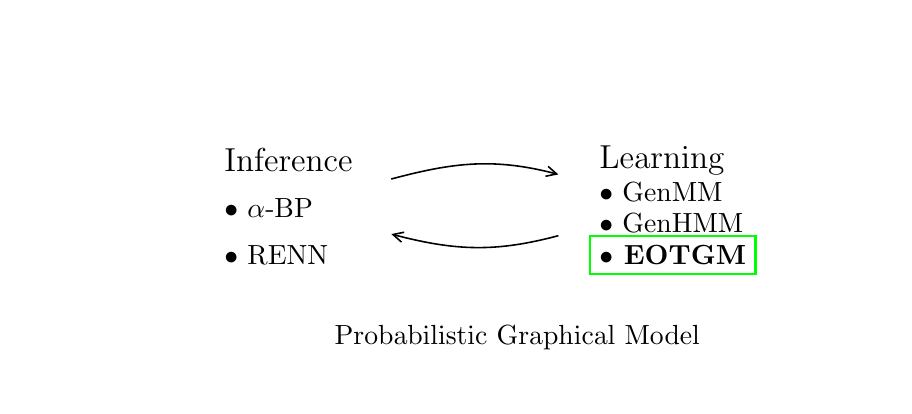
\begin{tikzpicture}
          \tikzstyle{cnode} = [thick, draw=white, ellipse, inner sep = 2pt,  align=center]
          \tikzstyle{fnode} = [thick, draw=white, ellipse, inner sep = 10pt,  align=center]
          \tikzstyle{rnode} = [thick, rectangle, inner sep = 1.5pt,  align=left]
          \node[rnode] (inf) at (-2, 0) {\large Inference};
          \node[rnode, below = 0.6cm of inf.west, anchor=west] (abp) {$\bullet$ {$\alpha$-BP}};
          \node[rnode, below = 1.2cm of inf.west, anchor=west] (renn) {$\bullet$ RENN};
          \node[cnode, fit=(abp)(inf)(renn)] (infn) {};
          
          \node[rnode, right = 3 of inf] (lern) {\large Learning};
          \node[rnode, below = 0.4 of lern.west, anchor=west] (genmm) {$\bullet$ GenMM};
          \node[rnode, below = 0.8 of lern.west, anchor=west] (genhmm) {{$\bullet$} GenHMM};
          \node[rnode, below = 1.2 of lern.west, anchor=west] (lfree) {\textbf{{$\bullet$} EOTGM}};
          \node[cnode, fit=(lern)(genmm)(genhmm)(lfree)] (learn) {};
          \node[rnode, draw=green, fit=(lfree)] () {};

          \node[fnode, fit=(infn)(lern)] (box) {};

          
          \node[below right = 0.5 and -0.5 of infn] {{Probabilistic} Graphical Model};
          \draw[->,line width=0.2mm] (infn) to[out=15, in=165] (learn);
          \draw[->,line width=0.2mm] (learn) to[out=195, in=-15] (infn);
        \end{tikzpicture}
      }
    \end{center}
    
  \end{frame}
}

%%% Local Variables:
%%% mode: latex
%%% TeX-master: "../ppgm_slide"
%%% End:



%%% Local Variables:
%%% mode: latex
%%% TeX-master: "../ppgm_slide"
%%% End:



%%%%%%%%%%%%%%%%%%%%%%%%%%%%%%%%%%%%%%%%%%%%%%%%%%%%%% 
% ------------------------------------------------
% Summary
%%%%%%%%%%%%%%%%%%%%%%%%%%%%%%%%%%%%%%%%%%%%%%%%%%%%%% 

\section{Summary and Q$\&$A}
\subsection{Summary}
\begin{frame}[label=current]{Summary}
  \begin{block}{Wrap-up}
  \begin{itemize}[label=$\bullet$]
  \item Inference with message-passing and analysis
  \item Inference with free energy minimization by neural networks
  \item Inference .. Learning: their interactions
  \item Neural network generators in EM for more flexible modeling; A Further step into temporal models
  \item A bonus modeling method for likelihood-free learning
  \end{itemize}
  \end{block}
\end{frame}
\subsection{Q$\&$A}

{ \setbeamercolor{background canvas}{bg=hl_bg}
  \setbeamercolor{normal text}{fg=hl_fg}
  \setbeamercolor{frametitle}{fg=hl_fg}
  \begin{frame}
    \usebeamercolor[fg]{normal text}
    \begin{center}
      {\large Thank you for your attention.}\\
      {\large Q$\&$A.}
    \end{center}
    
  \end{frame}
}


%%% Local Variables:
%%% mode: latex
%%% TeX-master: "../ppgm_slide"
%%% End:





\end{document}
%%% Local Variables:
%%% mode: latex
%%% TeX-master: t
%%% End:
